%\documentclass{article}
\documentclass
[   twoside=false,    
    fontsize=14pt,     
    DIV=15,           
    BCOR=17mm,         
    headsepline, 
    footsepline, 
    open=right,        
    paper=a4,          
    abstract=true,     
    listof=totoc,     
    bibliography=totoc,
    titlepage,       
    headinclude=true,  
    footinclude=false, 
    numbers=noenddot   
]   {scrreprt}      %scrreprt   

\usepackage[left=30mm, top=20mm, right=15mm, bottom=30mm]{geometry}
\sloppy
\usepackage{setspace}
\onehalfspacing 



%\usepackage[OT2,T2A,T2B,T1]{fontenc}

\usepackage[T2B]{fontenc}
%\usepackage[cp1251]{inputenc}
\usepackage[utf8]{inputenc}
\usepackage[english,russian]{babel}
\usepackage{amsmath,amssymb,amsfonts}  
\usepackage{setspace} 
\usepackage{bm} 
\usepackage{graphicx}  %  insert EPS  \includegraphics
\usepackage{psfrag} 
\usepackage{array}
\usepackage{caption}
\usepackage{hyperref}
\usepackage{stfloats}
\usepackage{textcomp}
\usepackage{tabulary}
\usepackage{float}
\usepackage{epstopdf}
\usepackage{misccorr}
\usepackage{times}
%\usepackage{mathptmx}
\usepackage{lmodern}
\usepackage[automark]{scrpage2}
\usepackage[active]{srcltx}


\makeatletter
\@addtoreset{equation}{chapter}
\@addtoreset{figure}{chapter}
\@addtoreset{table}{chapter}
\renewcommand\theequation{\thechapter.\@arabic\c@equation}
\renewcommand\thefigure{\thechapter.\@arabic\c@figure}
\renewcommand\thetable{\thechapter.\@arabic\c@table}
\makeatother

\setcounter{secnumdepth}{3} % Tiefe der Nummerierung
\setcounter{tocdepth}{3}    % Tiefe des Inhaltsverzeichnisses


% Seitenlayout festlegen. Hier nichts ?ndern!
\pagestyle{scrplain}
\ihead[]{}%\headmark}
\ohead[]{\pagemark}
\chead[]{}
\ifoot[]{}
\ofoot[]{}%\scriptsize \artderausarbeitung\ \namedesautors}
\cfoot[]{}
\renewcommand{\titlepagestyle}{scrheadings}
\renewcommand{\partpagestyle}{scrheadings}
\renewcommand{\chapterpagestyle}{scrheadings}
\renewcommand{\indexpagestyle}{scrheadings}


% Quelltextrahmen, klein. Hier nichts ?ndern!
\newsavebox{\inhaltkl}
\def\rahmenkl{\sbox{\inhaltkl}\bgroup\small\renewcommand{\baselinestretch}{1}\vbox\bgroup\hsize\textwidth}
\def\endrahmenkl{\par\vskip-\lastskip\egroup\egroup\fboxsep3mm%
\framebox[\textwidth][l]{\usebox{\inhaltkl}}}


% Quelltextrahmen, normale Groesse. Hier nichts ?ndern!
\newsavebox{\inhalt}
\def\rahmen{\sbox{\inhalt}\bgroup\renewcommand{\baselinestretch}{1}\vbox\bgroup\hsize\textwidth}
\def\endrahmen{\par\vskip-\lastskip\egroup\egroup\fboxsep3mm%
\framebox[\textwidth][l]{\usebox{\inhalt}}}


\newcommand{\bs}{\boldsymbol}
\newcommand{\compl}{\mathbb{C}}    
\newcommand{\real}{\mathbb{R}}  
\newcommand{\Amat}{\mathbf{A}}  
\newcommand{\Bmat}{\mathbf{B}}  
\newcommand{\amat}{\mathbf{a}}  
\newcommand{\bmat}{\mathbf{b}}  
\newcommand{\Camat}{\mathbf{C}^{[a]}}  
\newcommand{\Cbmat}{\mathbf{C}^{[b]}}  
\newcommand{\Xmat}{\mathbf{X}}  
\newcommand{\Xiten}{\mathcal{X}}  


\begin{document}
\selectlanguage{Russian}
\begin{singlespace}
%\documentclass[a4paper]{article}
%\usepackage[T1,OT2,T2B]{fontenc}
%\usepackage[cp1251]{inputenc}
%\usepackage[14pt]{extsizes} 
%\usepackage[russian]{babel}
%\usepackage{setspace,amsmath}
%\usepackage[left=20mm, top=15mm, right=15mm, bottom=15mm, nohead, footskip=10mm]{geometry} % настройки полей документа
%\usepackage{mathptmx}
%\usepackage{times}
%\begin{document} % начало документа
 
% НАЧАЛО ТИТУЛЬНОГО ЛИСТА
\begin{center}
\hfill \break
\large{МИНОБРНАУКИ РОССИИ}\\
\footnotesize{ФЕДЕРАЛЬНОЕ ГОСУДАРСТВЕННОЕ БЮДЖЕТНОЕ ОБРАЗОВАТЕЛЬНОЕ УЧРЕЖДЕНИЕ}\\ 
\footnotesize{ВЫСШЕГО ПРОФЕССИОНАЛЬНОГО ОБРАЗОВАНИЯ}\\
\small{\textbf{«КАЗАНСКИЙ НАЦИОНАЛЬНЫЙ ИССЛЕДОВАТЕЛЬСКИЙ НАУЧНЫЙ ТЕХНИЧЕСКИЙ УНИВЕРСИТЕТ им. А.Н. Туполева-КАИ»}}\\
\hfill \break
\normalsize{Институт радиоэлектроники и телекоммуникаций}\\
 \hfill \break
\normalsize{Кафедра радиоэлектронных и телекоммуникационных систем}\\
\hfill\break
\hfill \break
\hfill \break
\hfill \break
\hfill \break
\hfill \break
\hfill \break
\large{\textbf{Отчет}}\\
\normalsize{учебная практика}\\
\normalsize{Вид практики: преддипломная\\
\hfill \break
Направление  110402 Инфокоммуникационные технологии и системы связи
\hfill \break
Магистерская программа  Communication and signal processing\\
Срок практики с \underline{\hspace{3cm}} по \underline{\hspace{3cm}}}\\
\hfill \break
\hfill \break
\end{center}
 
 
\normalsize{ 
\begin{tabular}{cccc}
Отчет принял  с оценкой & \underline{\hspace{3cm}} &  \underline{\hspace{1cm}} &\underline{\hspace{3cm}} \\\\
Рук. пр. от КНИТУ-КАИ & \underline{\hspace{3cm}}& \underline{\hspace{1cm}}&\underline{\hspace{3cm}} \\\\
Обучающийся & \underline{\hspace{3cm}} & &Б.М.Валеев \\\\

\end{tabular}
}\\
\hfill \break
\hfill \break
\begin{center} Казань 2016 \end{center}
\thispagestyle{empty} % выключаем отображение номера для этой страницы
 
% КОНЕЦ ТИТУЛЬНОГО ЛИСТА
 
\newpage
 %
%\end{document}  % КОНЕЦ ДОКУМЕНТА !
\end{singlespace}
\onehalfspace
\pagenumbering{arabic} % Nummerierung der Seiten ab hier: i, ii, iii, iv...
\pagestyle{scrheadings} % Ab hier mit Kopf- und Fusszeile
\tableofcontents
%\clearpage
\newpage
\chapter{Введение}
В настоящее время радио частоты становятся все более дорогим ресурсом из-за большого количества работающих радиотехнических систем. Разумные пути для выделения радио ресурсов становятся все более и более важными в беспроводных технологиях. Методы совместного использования спектра являются одним из таких путей\cite{Book32}. Однако подобные технологии должны быть реализован очень аккуратно, для того что удерживать интерференцию на низком уровне для других легально работающих систем\cite{Book34}\cite{Book35}.  Четвертое поколение мобильной связи было основано на ОЧРК модуляции. Однако ОЧРК не предоставляло необходимого уровня межсистемной интерференции и недостаточно эффективно использовало радио ресурсы. Данный недостаток был связан с ортогональностью между всеми поднесущими частотами \cite{Book34} \cite{Book33}. В следующем поколении систем мобильной связи был предложен более эффективный путь для использования частотного ресурса. Новая техника названа Обобщенное частотное разделение каналов. Она основана на неортогональном расположении поднесущих частот. Передатчик располагает поднесущие частоты таким образом чтобы спектры данных работали с некоторым перекрытием между собой. Система обеспечивает такое поведение при помощи фильтров с характеристикой "Корень приподнятого косинуса" вместо использования согласованного фильтра. Выбранный подход позволяет уменьшить излучение вне рабочей полосы частот.Однако интерференция внутри системы значительно уменьшает производительность выбранного метода модуляции. При этом взаимное перекрытие в системе является настраиваемым параметром и таким образом система может выбирать компромисс между влиянием на чужие системы и производительностью своей системы. Так же новая система передачи данных значительно увеличивает сложность организации приемника. Это связано с тем что приемник обязан найти символы как во временной так и в частотной области.Данная задача имеет достаточно большую вычислительную сложность и увеличит размеры и энергопотребление приемного устройства. Более того для того чтобы обеспечить тот же уровень ошибок на бит приемник должен быть значительно сложнее и использовать совершенные алгоритмы расчета. При этом данную систему можно описать при помощи тензорной алгебры для того чтобы выразить ее в более естественной форме.
\section{Обработка сигналов основанная на тензорной алгебре}
Тензор это много размерный массив данных. Другими словами Н мерный тензор является матрицей у которой существуют элементы по Н разным измерениям\eqref{i_1}\cite{Book6}. Тензоры первого и второго порядка являются векторами и матрицами соответственно. Тензоры которые имеют количество измерений более двух считаются тензорами высоких порядков\cite{Book7}. 
\begin{align}
\mathcal{X} \in \compl^{I_1\times I_2\cdots I_N}
\label{i_1}
\end{align}
Порядок тензора это число измерений по которым тензор имеет различные элементы. В данной работе скалярные значения обозначены как прописные символы например $a$. Векторы обозначены как прописные символы полужирного шрифта например $\mathbf{a}$. Матрицы записаны как заглавные полужирные символы например $\mathbf{A}$. Тензоры высокого порядка обозначены как заглавные символы каллиграфического шрифта например $\mathcal{A}$. Тензоры позволяют описать данные в более естественной форме в случае если количество их естественных измерений больше двух. Описание данных при помощи тензоров позволяет учитывать многие зависимости между различными размерностями в данных. 
Развертка $N$-ого порядка является соединением тензора с фиксированной точкой одной размерности\eqref{i_2}\eqref{i_3}\eqref{i_4}\eqref{i_5}\cite{Book16}. При этом для каждого столбца все размерности за исключением одного являются фиксированными.  Развертка $N$-ого порядка имеет то же количество строк сколько имеет элементов по пространству v. Запись по столбцам может отличаться по порядку. Отличают запись по Матлаб и запись по Латауеру. Запись по Матлаб идет начиная от первого измерения к концу\cite{Book19}, в то время как по Латауеру от последнего измерения к первому. В данной работе используется запись по Матлаб во всех вычислениях, если явно не указано иное.
\begin{align}
\mathcal{X}_{:,:,1}=\begin{bmatrix}
1&3\\ 
0&1\\
\end{bmatrix} \; \mathcal{X}_{:,:,2}=\begin{bmatrix}
2&-3\\ 
-1&2\\
\end{bmatrix}
\label{i_2}
\end{align}
\begin{align}
\mathcal{X}_{[1]}=\begin{bmatrix}
1&3&2&-3\\ 
0&1&-1&2\\
\end{bmatrix}
\label{i_3}
\end{align}
\begin{align}
\mathcal{X}_{[2]}=\begin{bmatrix}
1&0&2&-1\\ 
3&1&-3&2\\
\end{bmatrix}
\label{i_4}
\end{align}
\begin{align}
\mathcal{X}_{[3]}=\begin{bmatrix}
1&0&3&1\\ 
2&-1&-3&2\\
\end{bmatrix}
\label{i_5}
\end{align}
$N$-мерный тензор имеет ранг один если он может быть представлен как внешнее произведение $N$ векторов\cite{Book6}. Разложение тензоров на тензоры ранга один было предложено Хичкоком в 1927 г\cite{Book5}. Он описал тензор высшего порядка как сумму тензоров ранга один. Тензор может быть разложен на некоторое количество тензоров ранга один. Такое разложение называют "Каноническое разложение" или "Параллельная факторизация"\eqref{i_6}\eqref{i_7}. Каноническое разложение раскладывает тензор на сумму тензоров ранга один. Данная сумма может быть представлена в иной форме.
\begin{align}
\mathcal{X}=\sum_{r=1}^R \mathbf{a}_r \circ \mathbf{b}_r \circ \mathbf{c}_r
\label{i_6}
\end{align}
\begin{align}
\mathcal{X}\in \compl^{I_1\times I_2\times I_3} \mathbf{a}_r\in \compl^{I_1\times 1} \mathbf{b}_r\in \compl^{I_2\times 1} \mathbf{c}_r\in \compl^{I_3\times 1}
\label{i_7}
\end{align} 
Векторы соответствующие тому же пространству при тензорах ранга один могут быть собраны в одну матрицу для каждой из размерностей\eqref{i_8}. Такая запись называется матричная факторизация. При помощи записанных матриц развертки каждого из порядков можно записать в значительно более простой форме\eqref{i_10}\eqref{i_11}\eqref{i_12}. 
\begin{align}
\mathcal{X}= \mathbf{A} \circ \mathbf{B} \circ \mathbf{C}
\label{i_8}
\end{align}
\begin{align}
\mathbf{A}=\begin{bmatrix}
\mathbf{a}_1&\mathbf{a}_2\cdots \mathbf{a}_R\\
\end{bmatrix}
\label{i_9}
\end{align}
\begin{align}
\mathcal{X}_{[1]}=\mathbf{A}(\mathbf{C}\diamond \mathbf{B})^T
\label{i_10}
\end{align}
\begin{align}
\mathcal{X}_{[2]}=\mathbf{B}(\mathbf{C}\diamond \mathbf{A})^T
\label{i_11}
\end{align}
\begin{align}
\mathcal{X}_{[3]}=\mathbf{C}(\mathbf{A}\diamond \mathbf{B})^T
\label{i_12}
\end{align}
Существует много путей разложить тензор, один из самых распространенных алгоритмов является метод ПМНК. Алгоритм описан ниже\cite{Book66}.
\begin{itemize}
\item Установка стартовых матриц $\mathbf{A,B,C}$ как случайных комплексных матриц фиксированного размера
\item  Решение СЛАУ с данными матрицами $\mathbf{B,C}$ и обновлением матрицы $\mathbf{A}$ 
\item Решение СЛАУ с данными матрицами $\mathbf{A,C}$ и обновлением матрицы $\mathbf{B}$ 
\item Решение СЛАУ с данными матрицами $\mathbf{A,B}$ и обновлением матрицы $\mathbf{C}$ 
\item Проверка уменьшения значения функции невязки. В случае если уменьшение больше порога, повторить с алгоритм с пункта 2.
\end{itemize}
\subsection{PARATUCK2}
Модель $PARATUCK2 $\cite{Book12} является комбинацией между $PARAFAC $\cite{Book6} и $TUCKER3$\cite{Book6} моделями разложения тензоров. Модель позволяет разложить один трехмерный тензор на 5 различных матриц. В общем случае модель может быть записана в скалярной форме при помощи следующего выражения\eqref{p_1} \cite{Book26}. 
\begin{align}
x_{i_1,i_2,t}=\sum^{F}_{f=1} \sum^{T_s}_{t_s=1}a_{i_1,f}c^{[a]}_{t,f}s_{f,t_s}c^{[b]}_{f,t_s}b_{i_2,t_s}
\label{p_1}
\end{align}
\begin{align*}
\mathcal{X} \in \compl^{I_1 \times, I_2 \times T} \mathbf{A} \in \compl^{I_1 \times F} \mathbf{B} \in \compl^{I_2 \times T_s}
\end{align*}
\begin{align*}
\mathbf{C}^{[a]} \in \compl^{T \times F} \mathbf{C}^{[b]} \in \compl^{T \times T_s}
\end{align*}
В указанном выше выражении $x_{i_1,i_2,t}$  является $(i_1,i_2,t)$  элементом тензора $\mathcal{X} \in \compl^{I_1 \times I_2 \times T }$. Матрица $\mathbf{S}$ является  матрицей-основой для $PARATUCK2$ модели. Матрицы $\mathbf{A}$ и $\mathbf{B}$ обеспечивают связь между соответствующей размерностью тензора $\mathcal{X}$ и  матрицы-основы $\mathbf{S}$\cite{Book12}. Матрицы $\Camat$ и $\Cbmat$ являются взвешивающими коэффициентами для матриц $\Amat$ и $\Bmat$ в каждом из слоев третьей размерности тензора $\Xiten$. 
Модель может быть записана в двух формах: послойная тензорная нотация\eqref{p_2} и векторизованная форма для тензора $\Xiten$.
В послойной форме записи тензор $\Xiten$ записывается отдельным выражением для каждого слоя третьей размерности.  Подобная запись позволяет описать модель при помощи линейной алгебры с минимальными изменениями в выражении для различных слоев. Матрицы $\Camat$ и $\Cbmat$ в таком случае записаны как тензор с элементами на главной диагонали между первым и вторым измерением. В таком случае послойная запись для модели $PARATUCK2 $ может быть выражена как послойное произведение между матрицей $\Amat$ и $\Bmat$ с коэффициентам для соответствующих строк и столбцов для матрицы$\Camat$ и $\Cbmat$ для соответствующего слоя третьего измерения\cite{Book12}.
\begin{align}
\mathbf{X}_{:,:,i}=\mathbf{A}\cdot diag(\mathbf{C^{[a]}}_{:,i})\cdot \mathbf{S}\cdot diag(\mathbf{C^{[b]}}_{:,i})\cdot \mathbf{B}
\label{p_2}
\end{align}
Векторизованная форма тензора $\Xiten$ является второй формой для записи модели. Возможно использовать данную запись в трех формах\cite{Book6}, в виде произведения матрицы с векторизованной матрицей $\Amat$ $\Bmat$ и $\mathbf{S}$. Таким образом можно найти каждую из матриц $\Amat$ $\Bmat$ и $\mathbf{S}$ используя векторизованную модель тензора $\Xiten$ и генерирующую матрицу для каждой из форм записи. Однако важно заметить, что векторизированная модель требует знания размерностей тензора $\Xiten$ так как вектор не позволяет узнать соответствующие размерности\cite{Book5}.
\begin{align}
vec(\mathcal{X})=\begin{bmatrix}
(\mathbf{C^{[a]T}} \diamond \mathbf{C^{[b]T}})^T \diamond (vec(A_{1,:})\otimes B)\\
(\mathbf{C^{[a]T}} \diamond \mathbf{C^{[b]T}})^T \diamond (vec(\mathbf{A}_{2,:})\otimes \mathbf{B})\\
\vdots \\
(\mathbf{C^{[a]T}} \diamond \mathbf{C^{[b]T}})^T \diamond (vec(\mathbf{A}_{I_1,:})\otimes \mathbf{B})\\
\end{bmatrix} vec(\mathbf{S})
\label{p_3}
\end{align}
\begin{align}
vec(\mathcal{X})=(\mathbf{I} \otimes(((\mathbf{B}\diamond \mathbf{C}^{[b]}) \cdot \mathbf{S}^T) \odot \mathbf{C}^{[a]}) )vec(\mathbf{A})
\label{p_4}
\end{align}
\begin{align}
vec(\mathcal{X})=(\mathbf{I} \otimes (((\mathbf{A}\diamond \mathbf{C}^{[a]}) \cdot \mathbf{S}) \odot \mathbf{C}^{[b]} ))vec(\mathbf{B})
\label{p_5}
\end{align}
Векторизированная модель записи может быть упрощена в случае если матрица $\Amat$ и матрица $\Bmat$ являются векторами,а не матрицами. В данном случае модель выраженная при помощи произведений Хатри-Рао и Адамара упрощаются до значительно меньшего количества операций, и произведение Кронекера исключается.
Упрощенная форма записывается для всех трех матриц в следующей форме.
\begin{align}
vec(\mathcal{X})^T=\mathbf{a}\cdot (\mathbf{C}^{[a]T} \odot (\mathbf{S}\cdot (\mathbf{C}^{[b]}\diamond \mathbf{b}^T)^T))
\label{p_6}
\end{align}
\begin{align}
vec(\mathcal{X})^T=\mathbf{b}^T\cdot (\mathbf{C}^{[b]T} \odot (\mathbf{S}^T  \cdot (\mathbf{C}^{[a]}\diamond \mathbf{a})^T))
\label{p_7}
\end{align}
\begin{align}
vec(\mathcal{X})=(((\mathbf{a}\diamond \mathbf{C}^{[a]}) \cdot \mathbf{S}) \odot \mathbf{C}^{[b]} )\mathbf{b})
\label{p_8}
\end{align}
\begin{align}
vec(\mathcal{X})=(((\mathbf{b}^T\diamond \mathbf{C}^{[b]}) \cdot \mathbf{S}^T) \odot \mathbf{C}^{[a]}) \mathbf{a}^T) 
\label{p_9}
\end{align}
\begin{align*}
\mathcal{X} \in \compl^{1 \times 1 \times T} 
\mathbf{a} \in \compl^{1 \times F} 
\mathbf{b} \in \compl^{T_s \times 1}
\end{align*}
\begin{align*}
\mathbf{C}^{[a]} \in \compl^{T \times F}
\mathbf{C}^{[b]} \in \compl^{T \times T_s}
\mathbf{S} \in \compl^{F \times T_s}
\end{align*}
Модель будет использована для описания выраженной ниже системы модуляции ОбЧРК. Данная модель позволяет описать систему передачи данных в достаточно простой форме. 
\section{Обобщенное частотное разделение каналов}
Основной принцип работы ОбЧРК является организация блока передачи в котором используется несколько поднесущих и несколько символов на каждой из поднесущих. При этом символы на поднесущих проходят низкочастотную фильтрацию для уменьшения межканальной интерференции. В системах с обобщенное частотное разделение каналов используется два основных вида фильтров во временной области: фильтр с характеристикой "Приподнятый косинус" либо фильтр с характеристикой корень приподнятого косинуса. В системе ортогонального частотного разделения каналов используется согласованный фильтр, обеспечивающий ортогональность различных поднесущих. В системах передачи данных с ОбЧРК поднесущие не ортогональны друг другу. По этой причине возникает наложение различных поднесущих друг на друга, что увеличивает меж символьную и меж канальную интерференцию. Однако подобный подход позволяет плотнее располагать поднесущие между собой и эффективнее использовать спектр.
\subsection{Принцип конструирования низкочастотного фильтра}
Как было сказано выше в ОбЧРК используется два основных вида фильтров во временной области: фильтр с характеристикой "Приподнятый косинус" либо фильтр с характеристикой корень приподнятого косинуса. Оба фильтра имеют одну переменную значение которой можно изменять для изменения перекрытия в частотной области между каналами $\alpha$. При этом значению переменной $\alpha=0$ соответствует минимальное перекрытие между соседними поднесущими, в то время как при значении $\alpha=1$ перекрытие является максимальным. При увеличении $\alpha$ значительно увеличивается меж-символьная и меж-канальная интерференция. В системе ОбЧРК происходит усложнение структуры приемника по сравнению с ОЧРК. Приемник должен обеспечивать прием даже в условиях меж-канальной интерференции и иметь механизмы для ее устранения.
Фильтр с характеристикой "Приподнятый косинус" является усовершенствованием согласованного фильтра, его характеристики широко освещены в литературе. Выражение для импульсной характеристики представлено в \eqref{g_1} и взято из источника \cite{Book17}. В выражении переменная $T$ является длительностью одного символа в шкале временных отсчетов, $\alpha$ как и было описано является переменной. Импульсная характеристика для для различных величин $\alpha$ представлена на рис. Соответствующая частотная характеристика для величин $\alpha$ представлена на рис. 
\begin{align}
\begin{matrix}
h(t)&=&\left\{
\begin{matrix}
\frac{\pi sinc(\frac{1}{2\alpha})}{4}& t=\pm \frac{T}{2\alpha}\\
sinc(1/T)\frac{cos(\pi \alpha t/T)}{1-(2 \alpha t /T)^2}&otherwise\\
\end{matrix} \right.
\end{matrix}
\label{g_1}
\end{align}
\begin{figure}[H]
\centering
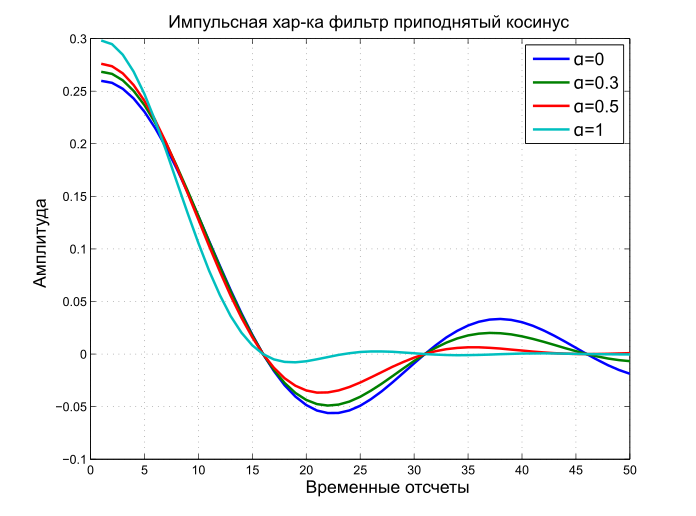
\includegraphics[width=0.9\columnwidth]{RC_time.png}
\caption{\textit{Импульсная характеристика фильтра типа Приподнятый косинус в зависимости от коэффициента $\alpha$}}
\label{fg_1}
\end{figure}
\begin{figure}[H]
\centering
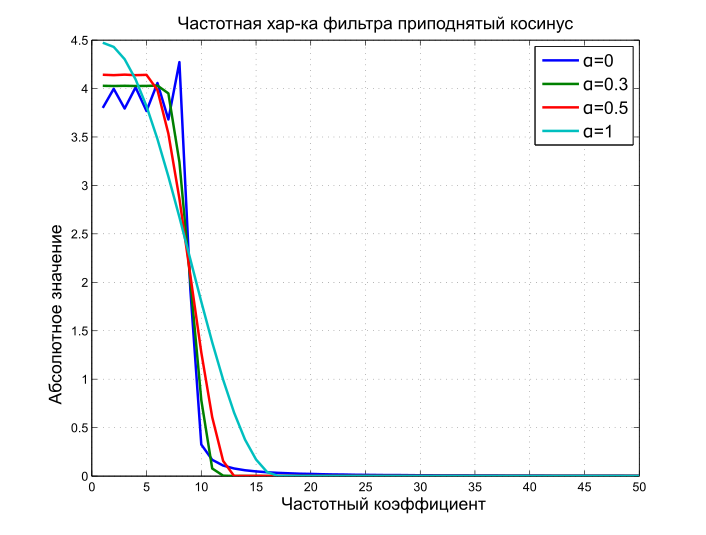
\includegraphics[width=0.9\columnwidth]{RC_freq.png}
\caption{\textit{Частотная характеристика фильтра Приподнятый косинус в зависимости от коэффициента $\alpha$}} 
\label{fg_2}
\end{figure}
Фильтр с характеристкой корень из приподнятого косинуса является дополнением к фильтру с характеристикой приподнятый косинус и при применении на приемнике и передатчике одновременно обеспечивает аналогичный уровень  межсимвольной интерференции как в согласованном фильтре. Описание и теоретическое обоснование использование фильтра описано в \cite{Book23} \cite{Book44} и \cite{Book51}. Выражение для импульсной характеристики представлено в \eqref{g_2} и взято из источника \cite{Book23}. В выражении переменная $T$ является длительностью одного символа в шкале временных отсчетов, $\alpha$ как и было описано является переменной. Импульсная характеристика для для различных величин $\alpha$ представлена на рис. Соответствующая частотная характеристика для величин $\alpha$ представлена на рис \eqref{fg_3}. 
\begin{figure}[H]
\centering
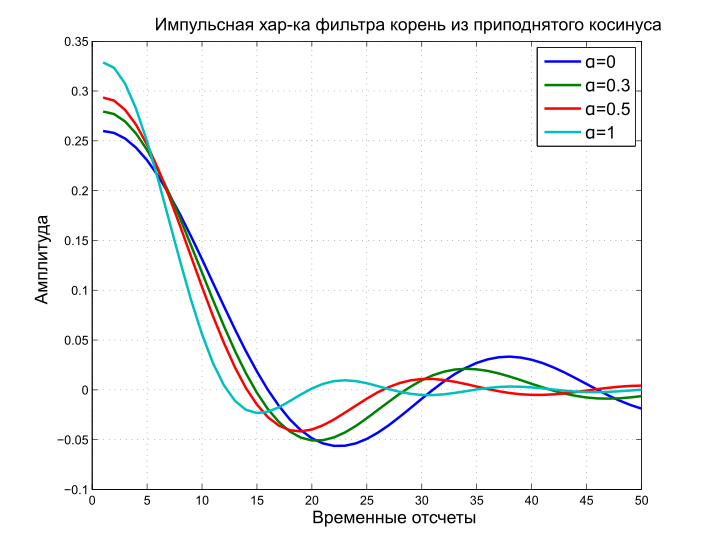
\includegraphics[width=0.9\columnwidth]{RRC_time.png}
\caption{\textit{Импульсная характеристика фильтра типа корень из Приподнятого косинуса в зависимости от коэффициента $\alpha$}} \label{fg_3}
\end{figure}
\begin{figure}[H]
\centering
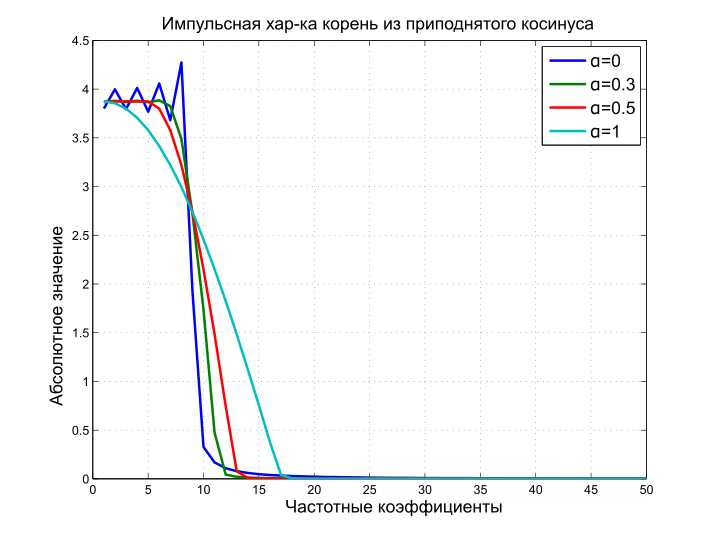
\includegraphics[width=0.9\columnwidth]{RRC_freq.png}
\caption{\textit{Частотная характеристика фильтра корень из Приподнятого косинуса в зависимости от коэффициента $\alpha$}} \label{fg_4}
\end{figure}
\begin{align}
\begin{matrix}
h(t) &=& \left\{ \begin{matrix} 
\frac{1-\alpha +4\alpha/\pi}{\sqrt{T}}& if& t=0\\
\frac{\alpha}{\sqrt{2T}}[(1+\frac{2}{\pi})sin(\frac{\pi}{4\alpha})+(1-\frac{2}{\pi})cos(\frac{\pi}{4\alpha})] & if &t= \pm T/4\alpha\\
\frac{1}{\frac{t\pi}{\sqrt{T}}(1-\frac{4*\alpha t}{T})^2}(sin(\frac{\pi t (1-\alpha)}{T})+\frac{4\alpha t}{T} cos(\frac{\pi t (1+ \alpha)}{T}) ) &otherwise \\
\end{matrix} \right.
\end{matrix}
\label{g_2}
\end{align}
Сравнение импульсных характеристик для согласованного фильтра, фильтра "Приподнятый косинус" и фильтра корень из приподнятого косинуса представлено на рис. Из рис.\eqref{fg_5} видно, что в точке где временной отсчет равен длительности импульса для согласованного фильтра амплитуда импульсной характеристики равна нулю, в отличие от других фильтров. Сравнение частотных характеристик для согласованного фильтра, фильтра "Приподнятый косинус" и фильтра корень из приподнятого косинуса представлено на рис. Из рис. видно, что для фильтра с характеристикой корень из приподнятого косинуса перекрытие по частоте является наибольшим в отличие от согласованного фильтра и фильтра с приподнятым косинусом.
\begin{figure}[H]
\centering
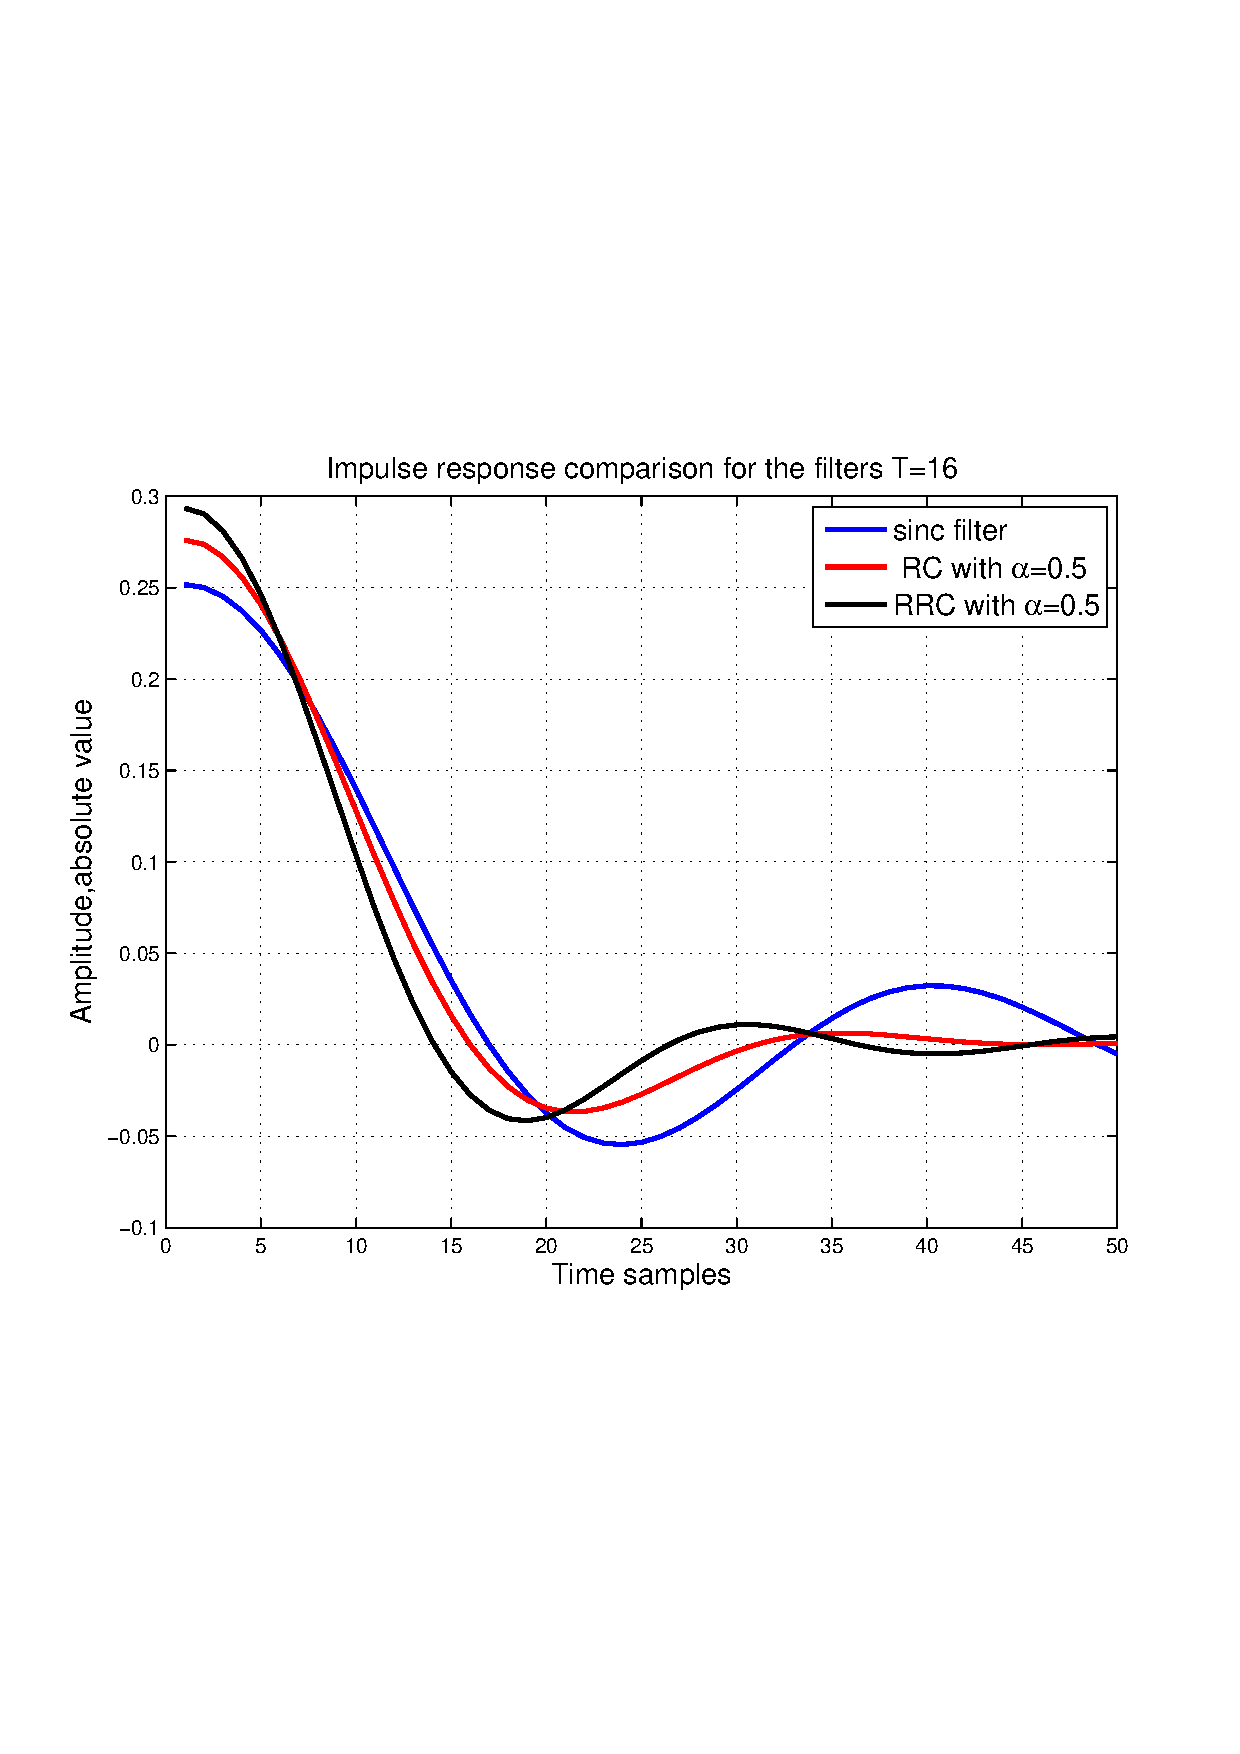
\includegraphics[width=0.9\columnwidth]{TIME_comp.png}
\caption{\textit{Сравнение импулсьных характеристик различных фильтров}} \label{fg_5}
\end{figure}
\begin{figure}[H]
\centering
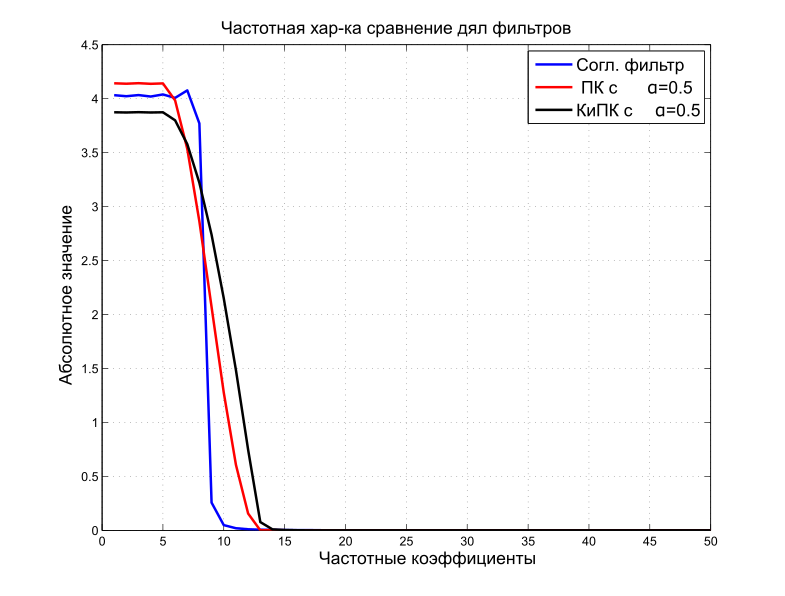
\includegraphics[width=0.9\columnwidth]{FREQ_comp.png}
\caption{\textit{С}} \label{fg_6}
\end{figure}
\section{Итеративный алгоритм с мягким порогом}
Одна из наиболее часто решаемых задач является задача деконволюции\cite{}. В матричной форме данная задача записывается как решение системы линейных алгебраических уравнений. Однако основной трудностью в решении СЛАУ является число обусловленности генерирующей матрицы\cite{Book66}. Увеличение числа обусловленности матрицы уменьшает стабильность решения СЛАУ. При этом число обусловленности является мультипликативным коэффициентом при погрешности вычисления\cite{Book55}. В классической постановке задача представлена на выражении \eqref{Book51} и может быть расписана следующим образом \eqref{ista_1}\cite{Book49}.
\begin{align}
R(x)=\mid\mid\mathbf{y}-\mathbf{Ax}\mid\mid^2_2 
\label{ista_1}
\end{align}
\begin{align}
R(x)=(\mathbf{y}-\mathbf{Ax})^H(\mathbf{y}-\mathbf{Ax})
\label{ista_2}
\end{align}
 В большинстве случаев для решения данной задачи используется обратная или псевдообратная матрица. В статье \cite{Book27} представлен итеративный алгоритм обеспечивающий сходимость к решению. При этом алгоритм гарантирует уменьшение функции невязки на каждой итерации. Основой и используемого алгоритма является "максимизация-минимизация". Подход позволяет заменить одну сложную задачу большим количеством простых задач. Каждая оптимизационная задача обеспечивает решение которое будет  находится ближе к решению задачи. На каждой итерации к исходной проблеме добавляется не отрицательное дополнительное слагаемое. Слагаемое должно быть таким, чтобы решаемая задача на данной итерации стала проще\cite{Book26}. Так же есть некоторые требования для дополнительного слагаемого $J_{add}(\mathbf{x})$ . Функция $J_{add}(\mathbf{x})$ должна удовлетворять выражению  $J_{add}(\mathbf{x})\geq R(\mathbf{x})$ для всех $\mathbf{x}$  и более того в точке $\mathbf{x}_k$ соответствующей текущему решению должно выполняться условие $J_{add}(\mathbf{x_k})= R(\mathbf{x_k})$.  Функциям $J_{add}(\mathbf{x})$ может быть различной на каждой итерации и должна обеспечивать простую минимизацию. Описанный ниже метод удовлетворяющий всем условиям назван "итерация  Ланвебера"\cite{Book24}. В оригинальной форме алгоритм написан для задач с действительными числами однако его можно расширить и для комплексных чисел. Определим $1$ как функция записанную в \eqref{ista_3}. В таком случае оптимизируемая функция будет записана в следующей форме $ R_1(\mathbf{x})$ \eqref{Book28} где $\alpha$ является коэффициентом для которого должно выполняться условие \eqref{ista_5}. Перепишем выражение раскрыв скобки и упростим его.
 
 \begin{align}
 \alpha \geq max(eig(\mathbf{A^HA}))
 \end{align}
 \begin{align}
 R(\mathbf{x_{k+1}})<R(\mathbf{x_k})
 \label{ista_3}
 \end{align}
\begin{align}
 R_1(\mathbf{x})=R(\mathbf{x})+J_{add}(\mathbf{x}) \label{ista_4}
\end{align}
\begin{align}
 R_1(\mathbf{x})=\mid\mid\mathbf{y}-\mathbf{Ax}\mid\mid^2_2+J_{add}(\mathbf{x})\label{ista_5}
\end{align}
\begin{align}
J_{add}(\mathbf{x})=(\mathbf{x-x_k})^T(\alpha \mathbf{I}-\mathbf{A}^T\mathbf{A})(\mathbf{x-x_k})\label{ista_6}
\end{align}
\begin{align}
 R_1(\mathbf{x})=\mid\mid\mathbf{y}-\mathbf{Ax}\mid\mid^2_2+(\mathbf{x-x_k})^H(\alpha \mathbf{I}-\mathbf{A}^H\mathbf{A})(\mathbf{x-x_k}) \label{ista_7}
\end{align}
\begin{align}
 R_1(\mathbf{x})=(\mathbf{y}-\mathbf{Ax})^H(\mathbf{y}-\mathbf{Ax})+(\mathbf{x}-\mathbf{x}_k)^H(\alpha \mathbf{I}-\mathbf{A}^H\mathbf{A})(\mathbf{x}-\mathbf{x}_k) \label{ista_8}
\end{align}
\begin{align}
\alpha \geq max(eig(\mathbf{A}^H\mathbf{A})) \label{ista_9}
\end{align}
\begin{align}
R_1(\mathbf{x})=\mathbf{y}^H\mathbf{y} -\mathbf{y}^H\mathbf{A}\mathbf{x} -\mathbf{x}^H \mathbf{A}^H\mathbf{y} +\mathbf{x}^H\mathbf{A}^H\mathbf{A}\mathbf{x} \label{ista_10}
\end{align}
\begin{align*}
 +\mathbf{x}_k^H(\alpha \mathbf{I}-\mathbf{A}^H\mathbf{A})\mathbf{x}_k +\mathbf{x}^H(\alpha \mathbf{I}-\mathbf{A}^H\mathbf{A})\mathbf{x} 
\end{align*}
\begin{align*}
-\mathbf{x}_k^H(\alpha \mathbf{I}-\mathbf{A}^H\mathbf{A})\mathbf{x} -\mathbf{x}^H(\alpha \mathbf{I}-\mathbf{A}^H\mathbf{A})\mathbf{x}_k 
\end{align*}
Описанная функция $ R_1(\mathbf{x})$ является вогнутой. Вогнутая функция имеет производную равную нулю в одной точке и эта точка является точкой минимума. Таким образом для нахождения точки минимума необходимо приравнять производную оптимизируемой функции к нулю и найти решение полученного уравнения. Поскольку функция является комплексной, она не аналитичная и от нее не существует аналитической производной. Для нахождения производной мы использовали  исчисление Виртингера\cite{Book27} и нашли производную по комплексно-сопряженной к искомой величине. В дальнейшем при упрощении выражения мы получаем в явном виде формулу для перехода от итерации к итерации \eqref{ista_11} позволяющую в конечном итоге привести производную оптимизируемой функции к нулю. Описанный алгоритм позволяет достичь линейной сходимости переменной $\mathbf{x}_k$, а так же уменьшить вычислительные затраты на работу алгоритма\cite{Book24}. 
\begin{align}
\frac{\delta R_1(x)}{\delta x^*}=-\mathbf{A}^H\mathbf{y} +\mathbf{A}^H\mathbf{A}\mathbf{x} +(\alpha \mathbf{I}-\mathbf{A}^H\mathbf{A})\mathbf{x} -(\alpha \mathbf{I}-\mathbf{A}^H\mathbf{A})\mathbf{x}_k \label{ista_11}
\end{align}
\begin{align}
\frac{\delta R_1(x)}{\delta x^*}=-\mathbf{A}^H\mathbf{y} +\alpha\mathbf{x} -\alpha\mathbf{x}_k+\mathbf{A}^H\mathbf{A}\mathbf{x}_k=0 \label{ista_12}
\end{align}
\begin{align}
\mathbf{A}^H(\mathbf{y} -\mathbf{A}\mathbf{x}_k) +\alpha\mathbf{x}_k =\alpha\mathbf{x} \label{ista_13}
\end{align}
\begin{align}
\mathbf{x}=\frac{\mathbf{A}^H}{\alpha}(\mathbf{y} -\mathbf{A}\mathbf{x}_k) +\mathbf{x}_k \label{ista_14}
\end{align}
\begin{align}
\mathbf{x}_{k+1}=\frac{\mathbf{A}^H}{\alpha}(\mathbf{y} -\mathbf{A}\mathbf{x}_k) +\mathbf{x}_k \label{ista_15}
\end{align}
К описанному алгоритму существует усовершенствование позволяющее достичь квадратичной сходимости без значительного увеличения вычислительной стоимости. Кроме того модификация описанного алгоритма позволяет решать задачу сжатого считывания путем использования мягкого порога около нулевого значения\cite{Book28}.
\begin{itemize}
\item Установить начальную точку $\mathbf{x}_0$ и установить промежуточные переменные $t_0=1, t_1=1$
\item Установить $\mathbf{y}_1=\mathbf{x}_0$
\item Обновить значение $t_1$ при помощи выражения \eqref{ista_16}
\item Найти решение выражение \eqref{ista_17} для итерации 
\item Установить $t_0=t_1$
\item Обновить промежуточную переменную при помощи выражения \eqref{}
\item Проверить, если величина шага на итерации меньше чем заданный порог. Если шаг больше, повторить операция с шага 3
\end{itemize}
\begin{align}
t_1=\frac{1+\sqrt{1+4t_1}}{2} \label{ista_16}
\end{align}
\begin{align}
\mathbf{x}_{k+1}=\frac{\mathbf{A}^H}{\alpha}(\mathbf{Y} -\mathbf{A}\mathbf{x}_k) +\mathbf{x}_k+\frac{t_0-1}{t_1}\cdot (\mathbf{x}_k-\mathbf{x}_{k-1}) \label{ista_17}
\end{align}
\clearpage
\chapter{ОбЧРК в системе с одной передающей и одной приемной антенной}
\section{Модель системы}
В данном разделе будет рассмотрена модель системы ОбЧРК. Была рассмотрена система передачи с воздействием канала. Канал в физическом смысле полагается как компоненты многолучевого распространения между передатчиком и приемником\cite{}. Так же канал может быть описан как свертка между переданным сигналом и некоторой импульсной характеристикой. В таком случае поступивший на вход приемника сигнал может быть описан следующим образом \eqref{siso_1}, где $y$ является вектором поступивших на вход приемника данных, $x$ это вектор переданных с выхода передатчика данных и $H$ это матрица свертки между входными данными и некоторой импульсной характеристикой. При этом переданный с выхода передатчика сигнал может быть связан с передаваемыми символами при помощи модели $PARATUCK2$ и ее двумя формами записи в векторизированной форме \eqref{siso_2}\eqref{siso_3}\cite{Book21}. 
\begin{align}
\mathbf{y}=\mathbf{Hx}
\label{siso_1}
\end{align}
\begin{align*}
\mathbf{y,x}\in\compl^{T\times 1}
\mathbf{H}\in\compl^{T\times T}
\end{align*}
\begin{align}
\mathbf{x}=\mathcal{X}_{[3]}=vec(\mathcal{X})=\mathbf{\Omega}_1 vec(\mathbf{S})
\label{siso_2}
\end{align}
\begin{align*}
\mathbf{\Omega}_1 \in \compl^{T\times T_s \cdot F}
\end{align*}
\begin{align}
\mathbf{\Omega}_1=(\mathbf{C}^{[b]T}\diamond \mathbf{C}^{[a]T})^T \diamond (\mathbf{b^T \otimes a}) \
\end{align}
\begin{align}
\mathcal{X}_{:,:,i}=\mathbf{a}\cdot diag(\mathbf{C}^{[a]}_{:,i})\cdot \mathbf{S} \cdot diag(\mathbf{C}^{[b]}_{:,i}) \cdot \mathbf{b} \label{siso_3}
\end{align}
Переданные данные могут быть сгенерированы при помощи модели $PARATUCK2$ третьего порядка в векторизованной форме или развертке третьего измерения. В таком случае матрица символов передаваемых при помощи системы передачи ОбЧРК будет записана как матрица основа $\mathbf{S}$ в модели $PARATUCK2$\cite{Book6}\eqref{siso_4}\eqref{siso_5}. Таким образом можно без изменений внести все символы в систему передачи. 

Каждый столбец в $\Camat$ матрице соответствует определенной поднесущей частоте для модуляции. Таким образом матрица $\Camat$ конструируется как значения поднесущих частот в каждом из столбцов. Таким образом матрица $\Camat$ может быть записана следующим образом \eqref{siso_1}.
 \begin{align}
 c^{[a]}_{t,f}=e^{-j2\pi\cdot(t\cdot f)/T_s} \label{siso_4}
 \end{align}
\begin{align}
\mathbf{C}^{[a]}=\begin{bmatrix}
e^{-j2\pi\cdot 0}& e^{-j2\pi\cdot 0}& \cdots & e^{-j2\pi\cdot 0} \\
e^{-j2\pi\cdot 0}& e^{-j2\pi\cdot 1/T_s}& \cdots &e^{-j2\pi\cdot F/T_s} \\
e^{-j2\pi\cdot 0}& e^{-j2\pi\cdot 2/T_s}& \cdots &e^{-j2\pi\cdot 2F/T_s} \\
&&\vdots \\
e^{-j2\pi\cdot 0}& e^{-j2\pi\cdot T/T_s}& \cdots & e^{-j2\pi\cdot T\cdot F /T_s} \\
\end{bmatrix} \label{siso_5}
\end{align}
Каждый столбец матрицы $\Cbmat$ определяет функцию фильтрации во временной области для заданного блока данных. Столбцы являются сдвинутыми версиями первого столбца. Сдвиг между соседними столбцами равен $T/T_s$\eqref{siso_7}. Элементы в столбце определяются по следующему выражению \eqref{siso_6}\cite{Book12}. При конструировании матрицы $\Cbmat$ задается коэффициент перекрытия $\alpha$.
\begin{align}
\begin{matrix}
u(t) &=& \left\{ \begin{matrix} 
\frac{1-\alpha +4\alpha/\pi}{\sqrt{T}}& if& t=0\\
\frac{\alpha}{\sqrt{2T}}[(1+\frac{2}{\pi})sin(\frac{\pi}{4\alpha})+(1-\frac{2}{\pi})cos(\frac{\pi}{4\alpha})] & if &t= \pm T/4\alpha\\
\frac{1}{\frac{t\pi}{\sqrt{T}}(1-\frac{4*\alpha t}{T})^2}(sin(\frac{\pi t (1-\alpha)}{T})+\frac{4\alpha t}{T} cos(\frac{\pi t (1+ \alpha)}{T}) ) &otherwise \\
\end{matrix} \right.
\end{matrix}\label{siso_6}
\end{align}
\begin{align}
\mathbf{C}^{[b]}=\begin{bmatrix}
\mathbf{u}_{0}& \mathbf{u}_{1}& \cdots &\mathbf{u}_{T_s}\\
\end{bmatrix} \label{siso_7}
\end{align}
Матрица $\Bmat$ при моделировании ОбЧРК становится столбцом $\bmat$ и в физическом смысле соответствует изменению по амплитуде между символами на различных временных позициях\cite{Book34}. Поскольку мы рассматриваем линейную независимую от времени систему то все значения в столбце равны единице. Кроме того таким образом можно выразить различные взвешивающие коэффициенты позволяющие не передавать символы по определенным временным позициям\eqref{siso_8}.
\begin{align}
\mathbf{b}=\mathbf{1}_{T_s\times 1} \label{siso_8}
\end{align}
\begin{align}
\mathbf{b}\in \real^{T_s\times 1} \label{siso_9}
\end{align}
Матрица $\Amat$ при моделировании GFDM становится строкой $\amat$ и в физическом смысле соответствует коэффициентам передачи для каждой поднесущей в течении одного блока передачи. В данной работе будет рассмотрена система где значения а могут быть структурированы двумя образами\eqref{siso_10}. В первом случае строка а имеет все единичные значения. Во втором случае величины в строке а могут быть распределены случайным образом между значениями $1$ и $0$. Так же при помощи строки $\amat$ может быть   аппроксимировано влияние канала. Однако точность такой аппроксимации мала.
\begin{align}
\mathbf{a}=\mathbf{1}_{1\times F} \label{siso_10}
\end{align}
\begin{align}
\mathbf{a}\in \compl^{1\times F} \label{siso_11}
\end{align}
Определив указанным образом соответствующие матрицы, сигнал на выходе передатчика может быть определен при помощи одного из последующих выражений \eqref{siso_13} \eqref{siso_14}. При этом модель системы ОбЧРК может быть совпадает с тензорной моделью $PARATUCK2$.
\begin{align}
\mathbf{x}^T=\mathbf{a}\cdot (\mathbf{C}^{[a]T} \odot (\mathbf{S}\cdot (\mathbf{C}^{[b]}\diamond \mathbf{b}^T)^T)) \label{siso_12}
\end{align}
\begin{align}
\mathbf{x}=((\mathbf{a}\diamond \mathbf{C}^{[a]})^T \cdot \mathbf{S}) \odot \mathbf{C}^{[b]} \mathbf{b}) \label{siso_13}
\end{align}
\begin{align}
\mathbf{x}=((\mathbf{b}^T\diamond \mathbf{C}^{[b]})^T \cdot \mathbf{S}^T) \odot \mathbf{C}^{[a]T} \mathbf{a}^T) \label{siso_14}
\end{align}
\begin{align*}
\mathbf{x} \in \compl^{T\times 1 }
\mathbf{a} \in \compl^{1\times F}
\mathbf{C}^{[a]} \in \compl^{T\times  F}
\end{align*}
\begin{align*}
\mathbf{C}^{[b]} \in \compl^{T \times T_s}
\mathbf{b} \in \compl^{T_s\times 1}
\mathcal{S} \in \compl^{F\times T_s }
\end{align*}
\section{Канал с аддитивным белым гауссовым шумом}
В данной секции будет рассмотрена модель системы в которой канал отсутствует, либо его влияние устранено.  В таком случае матрица $H$  из матрицы свертки преобразуется в единичную матрицу\cite{Book30}, а модель будет описана при помощи следующего выражения \eqref{siso_15}. Для подобного рода систем существует два классических решения.
\begin{align}
\mathbf{y}=\mathbf{\Omega}_1vec(\mathbf{S})+\mathbf{n} \label{siso_15}
\end{align}
\begin{align*}
\mathbf{\Omega}_1 \in \compl^{T\times T_s \cdot F}
\end{align*}
\begin{align}
\mathbf{\Omega}_1=(\mathbf{C}^{[b]T}\diamond \mathbf{C}^{[a]T})^T \diamond (\mathbf{b \otimes a})
\end{align}
\begin{align*}
\mathbf{y,n}\in \compl^{1\times T}
\mathbf{S}\in \compl^{F\times T_s}
\end{align*}
\begin{align*}
\mathbf{a} \in \compl^{1\times F}
\mathbf{C}^{[a]} \in \compl^{T\times  F}
\mathbf{C}^{[b]} \in \compl^{T \times T_s}
\mathbf{b} \in \compl^{T_s\times 1}
\end{align*}
\subsection{Приемник на основе псевдообратной матрицы}
Первое решение заключается оптимального решения с точки зрения второй нормы\cite{Book11}.  Для начала введем матрицу $\mathbf{\Omega}_1$ которая будет выражать взаимосвязь между векторизированной матрицей символов и сигналом на выходе передатчика\eqref{siso_ls_1}. Данное выражение может быть выведено из \eqref{siso_ls_3}. Приемник может найти наилучшие значения переданных данных при помощи решения задачи оптимизации\cite{Book26}. В таком случае может быть составлена следующая функция невязки \eqref{siso_ls_4}. Поскольку используется вторая норма, решение данной задачи существует и оно единственно. В случае если векторы а и б имеют структуру со всеми единицами мы можем ими пренебречь. Тогда матрица $\Omega$ будет записана как произведение Хатри-Рао между матрицами $\Camat$ и $\Cbmat$\eqref{siso_ls_4}.
\begin{align}
vec(\mathbf{x})=\mathbf{\Omega}_1\cdot vec(\mathbf{\widehat{S}}) \label{siso_ls_1}
\end{align}
\begin{align*}
\mathbf{\Omega}_1 \in \compl^{T\times T_s \cdot F}
\end{align*}
%\mathbf{\Omega}_3 \in \compl^{T\times T_s}
%\mathbf{\Omega}_2 \in \compl^{T\times F}
%vec(\mathbf{a}) \in \compl^{F \times 1}
\begin{align*}
vec(\mathbf{\widehat{S}}) \in \compl^{F \cdot T_s \times 1}
\end{align*}
\begin{align}
\mathbf{\Omega}_1=(\mathbf{C}^{[b]T}\diamond \mathbf{C}^{[a]T})^T \diamond (\mathbf{b \otimes a}) \label{siso_ls_2}
\end{align}
\begin{align}
\mathbf{\Omega}_1=(\mathbf{C}^{[b]T}\diamond \mathbf{C}^{[a]T})^T  \label{siso_ls_3}
\end{align}

\begin{align}
r_1= \mathbf{y}-\mathbf{\Omega}_1 \cdot vec(\mathbf{\widehat{S}})  \label{siso_ls_4}
\end{align}

Для того чтобы найти оптимальное решение возьмем первую производную от оптимизируемой функции\eqref{siso_ls_5}\cite{Book24}. Поскольку она комплексна и не аналитична, используем  исчисление Виртингера\eqref{siso_ls_6}, для того чтобы взять производную по комплексно сопряженной от переменной. Приравняем первую производную нулю и решим задачу используя псевдообратную матрицу\eqref{siso_ls_10}\cite{Book24}.
\begin{align}
\min_{vec(\mathbf{\widehat{S}})} r_1^H\cdot r_1=\min_{vec(\mathbf{\widehat{S}})} \mid\mid r_1\mid\mid^2  \label{siso_ls_5}
\end{align}
\begin{align}
r_1^H\cdot r_1=(vec(\mathbf{y})-\mathbf{\Omega}_1 \cdot vec(\mathbf{\widehat{S}}))^H\cdot(vec(\mathbf{y})-\mathbf{\Omega}_1 \cdot vec(\mathbf{\widehat{S}}))  \label{siso_ls_6}
\end{align}
\begin{align*}
r_1^H\cdot r_1=\mid\mid vec(\mathbf{y})\mid\mid^2 + vec(\mathbf{\widehat{S}})^H\mathbf{\Omega}_1^H \mathbf{\Omega}_1 vec(\mathbf{\widehat{S}}) 
\end{align*}
\begin{align}
-vec(\mathbf{y})^H \mathbf{\Omega}_1 vec(\mathbf{\widehat{S}})- vec(\mathbf{\widehat{S}})^H\mathbf{\Omega}_1^Hvec(\mathbf{y}) \label{siso_ls_7}
\end{align}
\begin{align}
\frac{\delta r_1^H\cdot r_1}{\delta vec(\mathbf{\widehat{S}}^*)} = \mathbf{\Omega}_1^H \mathbf{\Omega}_1 vec(\mathbf{\widehat{S}}) -\mathbf{\Omega}_1^Hvec(\mathbf{y})=0  \label{siso_ls_8}
\end{align}
\begin{align}
\mathbf{\Omega}_1^H \mathbf{\Omega}_1 vec(\mathbf{\widehat{S}})=\mathbf{\Omega}_1^Hvec(\mathbf{y}) \label{siso_ls_9}
\end{align}
\begin{align}
vec(\mathbf{\widehat{S}})_{opt}= (\mathbf{\Omega}_1^H \mathbf{\Omega}_1)^{-1}\mathbf{\Omega}_1^Hvec(\mathbf{y})  \label{siso_ls_10}
\end{align}
\subsection{Приемник на основе согласованного фильтра}
Существует другое решение задачи обеспечивающее более стабильное решение. Псевдообратная матрица имеет значительный недостаток в случае если матрица для которой осуществляется инверсия имеет плохое число обусловленности\cite{Book25}\eqref{siso_mf_1}. В таком случае если в принятых данных присутствует белый гауссов шум, его компоненты будут увеличены по мощности, что приведет к уменьшение соотношения $SNR$. Это можно легко увидеть используя разложение матрицы на собственные значения\eqref{siso_mf_2}\cite{Book25}. В таком случае обратная матрица к исходной будет записана следующим образом \eqref{siso_mf_4}. Как видно из выражения \eqref{siso_mf_4} при умножении вектора шума на матрицу обратную к $\mathbf{\Omega}_1$ происходит умножение собственных значений шума на  величины обратные к собственным значениям матрицы $\mathbf{\Omega}_1$\eqref{siso_mf_5}\cite{Book24}. Таким образом значения имеющие маленькую величину в обратной матрице обеспечат увеличение компонент шума\cite{}. Для того чтобы избежать подобного влияния можно произвести умножение на эрмитово сопряженную матрицу с исходной. В таком случае соотношение $SNR$ останется неизменным\eqref{siso_mf_6}. 
\begin{align}
\mathbf{\Omega}_1=\mathbf{U\Sigma V^H} \label{siso_mf_1}
\end{align}
\begin{align}
\mathbf{\Omega}_1^{-1}=\mathbf{V\Sigma^{-1} U^H} \label{siso_mf_2}
\end{align}
\begin{align}
\mathbf{n}=\mathbf{U I\delta^2 V^H} \label{siso_mf_3}
\end{align}
\begin{align}
E(\mathbf{\Omega}_1^{-1}\mathbf{n})=\mathbf{V(\Sigma^{-1}\cdot I\delta^2) V^H} \label{siso_mf_4}
\end{align}
\begin{align}
\mathbf{\Omega}_1^{H}=\mathbf{V\Sigma U^H} \label{siso_mf_5}
\end{align}
\begin{align}
E(\mathbf{\Omega}_1^{H}\mathbf{n})=\mathbf{V(\Sigma\cdot I\delta^2) V^H} \label{siso_mf_6}
\end{align}

\section{Поиск коэффициентов передачи поднесущих}
Введенные выше коэффициенты $\mathbf{a}$ используются для выбора рабочих поднесущих в системе. Изменение значений вектора $\mathbf{a}$ может быть использовано для уменьшения интерференции с другими системами работающими в том же диапазоне частот, что и система ОбЧРК\cite{Book25}.  Таким образом значение вектора $\mathbf{a}$ может быть неизвестным для приемника. Информация о коэффициенте передачи поднесущей должна быть дополнительным образом найдена на приемнике. Рассмотренная модель может быть описана при помощи модели $PARATUCK2$ третьего порядка\eqref{siso_s_1}.
\begin{align}
\mathbf{y}=\mathbf{\Omega}_1vec(\mathbf{S})+\mathbf{n} \label{siso_s_1}
\end{align}
 Тогда вектор $\mathbf{a}$ описывает коэффициент передачи каждой из поднесущей. Выражение \eqref{siso_s_2} может быть сформулировано относительно вектора $\mathbf{a}$ выписанного в правую часть. Таким образом можно записать уравнение невязки для искомого вектора $\mathbf{a}$\eqref{siso_s_3}. 
 \begin{align}
\mathbf{\Omega}_2=((\mathbf{C}^{[b]}\diamond \mathbf{b}^T)^T\cdot S^T) \odot \mathbf{C}^{[a]}   \label{siso_s_2}
\end{align}
\begin{align}
r_2= \mathbf{y}-\mathbf{\Omega}_2 \cdot vec(\mathbf{a})  \label{siso_s_3}
\end{align}

Приемник может найти как неизвестные величины вектора $\mathbf{a}$ так и переданные символы, но не в полном объеме. Поскольку в принятом на вход приемника блоке данных всего $T_s\cdot F$ величин, в то время как количество переменных равно $(T_s+1)\cdot F$ то задача является неопределенной и необходимо уменьшить количество неизвестных для решения задачи. Одним из возможных решений является определить для приемника первый символ на каждой из поднесущих, тогда количество неизвестных будет равно количество принятых на входи приемника данных и задача будет иметь как минимум одно решение. При помощи известных символов приемник сможет найти коэффициенты передачи поднесущих, после чего восстановит значения неизвестных для него символов\eqref{siso_sm_1}. Тогда для нахождения неизвестных величин должна быть сформулирована оптимизационная задача для приемника в ходе которой он сможет найти все неизвестные. Неизвестными переменными являются матрица символов $\mathbf{S}$ и вектор коэффициентов поднесущих $\mathbf{a}$. Известный символы добавлены в оптимизируемую функцию в качестве ограничения. Данный подход увеличивает вычислительную сложность задачи, однако значительно упрощает ее решение. Подобную задачу можно решить путем множителей Лагранжа. Задача была решена добавлением второй нормы от ограничения в функцию минимизации. Таким образом задача была упрощена с аналитической точки зрения однако так же усложнения с точки зрения вычислительной сложности. Кроме того было использовано два подхода по рассмотрению связи между невязками $r_1$ и $r_2$. Мы рассматривали как равенство функций $r_1$ и $r_2$ в той же самой точке, как и отсутствие связи между ними. В случае если связь отсутствует, производная по $\mathbf{S}$ и $\mathbf{a}$ равна нулю. В случае если связь присутствует производная по $\mathbf{S}$ и $\mathbf{a}$  не равна нулю.Далее будут рассмотрены оба подхода к решению оптимизационной задачи.
\subsection{Приближенный полу-слепой приемник}
Описанный ниже способ решения подразумевает отсутствие связи между $r_1$ и $r_2$. Постановка задачи записана в выражении \eqref{siso_sm_2}. Происходит минимизация функции с предположением что две оптимизируемые функции не зависят друг от друга.
\begin{align*}
\mathbf{r}_1= vec(\mathbf{y})-\mathbf{\Omega}_1 \cdot vec(\mathbf{\widehat{S}})
\end{align*}
 Функция невязки $r_1$ соответствует оптимизируемой функции относительно символов.  Матрица $\mathbf{\Omega}_1$ была определена ранее.
Функция невязки $r_2$ соответствует оптимизируемой функции относительно коэффициентов поднесущих. Матрица $\mathbf{\Omega}_2$ была определена ранее и соответствует переданным данным с выраженными из матрицы коэффициентами поднесущих.
 \begin{align*}
\mathbf{r}_2=vec(\mathbf{y})-\mathbf{\Omega}_2 \cdot vec(\mathbf{\widehat{s}})
\end{align*}
Функция невязки соответствует поставленному для алгоритма ограничению. В качестве матрицы выбора использована матрица $\mathbf{S}_{sel}$. В матрице $\mathbf{S}_{sel}$ присутствуют элементы только на главной диагонали и только в тех строках для которых переданный символ известен. Так же матрицу можно получить другим способом при помощи выражения.

 Вектор $\mathbf{q}$ является вектором где присутствуют известные символы, при этом от имеет ту же размерность что и вектор символов и на неизвестных позициях элементы равны нулю.
 \begin{align}
\mathbf{r}_3=\mathbf{q} -\mathbf{S}_{sel} vec(\mathbf{\widehat{S}}); \label{siso_sm_1}
\end{align}
\begin{align*}
\mathbf{S}_{sel}=diag(\mathbf{q})^{-1}diag(\mathbf{q})
\end{align*}
\begin{align*}
\mathbf{q}\in \compl^{T_s \cdot F\times 1}
\mathbf{S}_{sel}\in \compl^{T_s \cdot F\times T_s \cdot F} 
\end{align*}
\begin{align*}
\mathbf{r}_1 \in \compl^{T_s \cdot F \times 1}
\mathbf{r}_2 \in \compl^{F \times 1}
\mathbf{r}_3 \in \compl^{T_s \cdot F \times 1}
\end{align*}
\begin{align}
\min_{vec(\mathbf{\widehat{S}})} r_1^Hr_1 \label{siso_sm_2}
\end{align}
\begin{align}
\min_{vec(\mathbf{a})} r_2^Hr_2 \label{siso_sm_3}
\end{align}
\begin{align}
\min_{vec(\mathbf{\widehat{S}})} r_3^Hr_3 \label{siso_sm_4}
\end{align}
\begin{align}
\begin{bmatrix}
\frac{\delta \mathbf{r}_1^H \mathbf{r}_1}{\delta vec(\mathbf{\widehat{S}})^*}\\
\frac{\delta \mathbf{r}_2^H \mathbf{r}_2}{\delta vec(\mathbf{\widehat{a}})^*}\\
\frac{\delta \mathbf{r}_3^H \mathbf{r}_3}{\delta vec(\mathbf{\widehat{S}})^*}\\
\end{bmatrix}=
\begin{bmatrix}
0\\
0\\
0\\
\end{bmatrix} \label{siso_sm_5}
\end{align}
\begin{align}
\begin{bmatrix}
\frac{\delta \mathbf{r}_1^H \mathbf{r}_1}{\delta vec(\mathbf{\widehat{S}})^*}\\
\frac{\delta \mathbf{r}_2^H \mathbf{r}_2}{\delta vec(\mathbf{\widehat{S}})^*}\\
\frac{\delta \mathbf{r}_3^H \mathbf{r}_3}{\delta vec(\mathbf{\widehat{S}})^*}\\
\end{bmatrix}=
\begin{bmatrix}
-\mathbf{\Omega}_1^H \mathbf{r}_1\\
-\mathbf{\Omega}_2^H \mathbf{r}_2\\
-\mathbf{S}_{sel}^H \mathbf{r}_3\\
\end{bmatrix} \label{siso_sm_6}
\end{align}
\begin{align}
\frac{\delta r_1^Hr_1}{\delta vec(\mathbf{\widehat{S}}^*)} = \mathbf{\Omega}_1^H \mathbf{\Omega}_1 vec(\mathbf{\widehat{S}}) -\mathbf{\Omega}_1^Hvec(\mathbf{y})=0 \label{siso_sm_7}
\end{align}
\begin{align}
\frac{\delta r_2^Hr_2}{\delta vec(\mathbf{\widehat{a}}^*)} = \mathbf{\Omega}_2^H \mathbf{\Omega}_2 vec(\mathbf{\widehat{a}}) -\mathbf{\Omega}_2^Hvec(\mathbf{y})=0 \label{siso_sm_8}
\end{align}
\begin{align}
\frac{\delta r_3^Hr_3}{\delta vec(\mathbf{\widehat{S}}^*)} =\mathbf{S}_{sel}^H \mathbf{S}_{sel} vec(\mathbf{\widehat{S}}) -\mathbf{S}_{sel}^Hvec(\mathbf{q})=0 \label{siso_sm_9}
\end{align}
\begin{align}
\mathbf{S}_{sel}^H \mathbf{S}_{sel}=\mathbf{S}_{sel} \label{siso_sm_10}
\end{align}
В выражениях \eqref{siso_sm_10}\eqref{siso_sm_9}\eqref{siso_sm_8} присутствует ноль, мы можем минимизировать сумму обоих выражений. Указанное выражение может быть трансформировано в систему нелинейных уравнений при умножении на $-1$. Мы рассмотрели два метода решения системы нелинейных уравнений.
\begin{itemize}
\item Перемежающийся метод наименьших квадратов\cite{Book66}
\item Метод Ньютона\cite{Book65}
\end{itemize}
Алгоритм ПМНК описан ниже и работает в следующем порядк\cite{Book66}:
\begin{itemize}
\item Установить начальную точку $\theta_0$
\item Решить уравнение \eqref{siso_sm_7} \eqref{siso_sm_9} по отношению к $vec(\mathbf{S})$ с фиксированным $\mathbf{A}$ и обновить таким образом  $vec(\mathbf{S})$
\item Решить уравнение \eqref{siso_sm_8} по отношению к $\mathbf{A}$ с фиксированным $vec(\mathbf{S})$ и обновить таким образом  $\mathbf{A}$
\item Проверить, было ли уменьшение функции невязки на величину меньшую чем порог. Если уменьшение было больше порога, повторить процесс.
\end{itemize}
Метод Ньютона включает в себя следующие шаги\cite{Book64}:
\begin{itemize}
\item Установить начальную точку $\theta_0$
\item Решить систему  линейных алгебраических уравнений \eqref{siso_sm_11} в точке $\theta_0$\eqref{siso_sm_12}.
\item Проверить, было ли уменьшение функции невязки на величину меньшую чем порог. Если уменьшение было больше порога, повторить процесс.
\end{itemize}
Приемник не может решить данную систему в одну итерацию и совершит некоторое количество итераций. Задача может быть плохо поставлена на некоторых итерациях в силу присутствия аддитивного шума в данных. Для устранения такого влияния были рассмотрены два дополнительных подхода для увеличения стабильности алгоритма:
\begin{itemize}
\item  Правило $Powell-Wolf$ для адаптации шага итерации\cite{Book62}\cite{Book63}
\item  Алгоритм $Levenberg-Marquadrt$ по регуляризации сходимости\cite{Book66}\cite{Book68}\eqref{siso_sm_11}
\end{itemize}
Основное решаемое уравнение метода Ньютона является решение системы линейных уравнений указанное на \eqref{siso_sm_18} В указанном выражении $F$ это уравнение минимизируемое до нуля\eqref{siso_sm_13}. Вектор $F$ является первой производной оптимизируемой функции. В качестве матрицы $J$ используется вторая производная оптимизируемой функции либо Якобиан вектора $F$\eqref{siso_sm_19}.
\begin{align}
\mathbf{J\theta}=-\mathbf{F} \label{siso_sm_11}
\end{align}
\begin{align}
\mathbf{\delta \theta}=-\mathbf{J^+d}
\label{siso_sm_111}
\end{align}
\begin{align}
\begin{bmatrix}
vec(\mathbf{\widehat{S}})\\
vec(\mathbf{\widehat{a}})\\
\end{bmatrix}^{k+1}= 
\begin{bmatrix}
vec(\mathbf{\widehat{S}})\\
vec(\mathbf{\widehat{a}})\\
\end{bmatrix}^{k}+ \alpha \mathbf{\theta} \label{siso_sm_12}
\end{align}
\begin{align*}
\alpha=(0;1]
\end{align*}
\begin{align}
\mathbf{F}=\begin{bmatrix}
\frac{\delta \mathbf{r}_1^H \mathbf{r}_1}{\delta vec(\mathbf{\widehat{S}})^*}\\
\frac{\delta \mathbf{r}_2^H \mathbf{r}_2}{\delta vec(\mathbf{\widehat{a}})^*}\\
\frac{\delta \mathbf{r}_3^H \mathbf{r}_3}{\delta vec(\mathbf{\widehat{S}})^*}\\
\end{bmatrix}=0 \label{siso_sm_13}
\end{align}
%\begin{align}
%\frac{\delta r_1^Hr_1}{\delta vec(\mathbf{S}^*)}+\frac{\delta r_2^Hr_2}{\delta vec(\mathbf{A}^*)}+\frac{\delta r_3^Hr_3}{\delta vec(\mathbf{S}^*)}=0
%\end{align}
\begin{align}
\mathbf{\Omega}_1^H \mathbf{\Omega}_1 vec(\mathbf{\widehat{S}}) -\mathbf{\Omega}_1^Hvec(\mathbf{y})+\mathbf{\Omega}_2^H \mathbf{\Omega}_2 vec(\mathbf{\widehat{a}})  \label{siso_sm_14}
\end{align}
\begin{align}
-\mathbf{\Omega}_2^Hvec(\mathbf{y})+\mathbf{S}_{sel} vec(\mathbf{\widehat{S}}) -\mathbf{S}_{sel}^Hvec(\mathbf{q})=0 \label{siso_sm_15}
\end{align}
\begin{align*}
\begin{bmatrix}
\mathbf{\Omega}_1&0 \\
0&\mathbf{\Omega}_2\\
\mathbf{S}_{sel}&0 \\
\end{bmatrix}^H 
\begin{bmatrix}
vec(\mathbf{y}) \\
vec(\mathbf{y})\\
\mathbf{q} \\
\end{bmatrix}-
\begin{bmatrix}
\mathbf{\Omega}_1&0 \\
0&\mathbf{\Omega}_2\\
\mathbf{S}_{sel}&0 \\
\end{bmatrix}^H
\begin{bmatrix}
\mathbf{\Omega}_1&0 \\
0&\mathbf{\Omega}_2\\
\mathbf{S}_{sel}&0 \\
\end{bmatrix}\begin{bmatrix}
vec(\mathbf{\widehat{S}})\\
vec(\mathbf{\widehat{a}})\\
\end{bmatrix} 
\end{align*}
\begin{align}
\begin{bmatrix}
\mathbf{S}_{sel}^Hvec(\mathbf{q})+\mathbf{\Omega}_1^Hvec(\mathbf{y}) \\
\mathbf{\Omega}_2^Hvec(\mathbf{y})\\
\end{bmatrix} \label{siso_sm_16}
\end{align}
\begin{align}
-\begin{bmatrix}
\mathbf{\Omega}_1^H \mathbf{\Omega}_1+ \mathbf{S}_{sel}& \mathbf{0}\\
\mathbf{0} & \mathbf{\Omega}_2^H \mathbf{\Omega}_2\\
\end{bmatrix} \cdot \begin{bmatrix}
vec(\mathbf{\widehat{S}})\\
vec(\mathbf{\widehat{a}})\\
\end{bmatrix} =\mathbf{F} \label{siso_sm_17}
\end{align}
Поскольку оптимизируемая функция \eqref{siso_sm_12} является аналитической мы не используем исчисление Виртингера и ищем частную производную по отношению к вектору $\theta$\cite{Book58}.
\begin{align}
\mathbf{J}=\frac{\delta \mathbf{F}}{\delta \mathbf{\theta}} \label{siso_sm_18}
\end{align}
\begin{align}
\mathbf{J}=-\begin{bmatrix}
\mathbf{\Omega}_1^H \mathbf{\Omega}_1+ \mathbf{S}_{sel}& \mathbf{0}\\
\mathbf{0} & \mathbf{\Omega}_2^H \mathbf{\Omega}_2\\ 
\end{bmatrix} \label{siso_sm_19}
\end{align} 
Приемник на каждой итерации решает систему линейных уравнений и обновляет искомый вектор для следующего шага. Оптимизационный алгоритм уменьшает функцию невязки и уменьшает первую производную до нуля. Поскольку вторая норма является вогнутой функцией, следовательно у оптимизируемой функции существует только одно решение.
\subsection{Полу-слепой приемник}
Оптимизируемая функция может быть записана в общей форме в отличии от того как это было описано ранее\eqref{siso_jsm_1}. Записанная обобщенная форма делает каждую итерацию вычислительно дороже. Следует заметить что функции $r_1$ и $r_2$ равны между собой в той же самой точке $\mathbf{a}$ и $\mathbf{S}$. Функции могут быть заменены между собой при условии что переменные обеих функции равны между собой. 
\begin{align*}
\mathbf{r}_1= vec(\mathbf{y})-\mathbf{\Omega}_1 \cdot vec(\mathbf{\widehat{S}})=\mathbf{r}_2 
\end{align*}
\begin{align*}
\mathbf{r}_2= vec(\mathbf{y})-\mathbf{\Omega}_2 \cdot vec(\mathbf{\widehat{a}})
\end{align*}
\begin{align*}
\mathbf{r}_3=\mathbf{q} -\mathbf{S}_{sel} vec(\mathbf{\widehat{S}});
\end{align*}
\begin{align}
vec(\mathbf{y})-\mathbf{\Omega}_1 \cdot vec(\mathbf{\widehat{S}}_1)= vec(\mathbf{y})-\mathbf{\Omega}_2 \cdot vec(\mathbf{\widehat{a}}_1)  \label{siso_jsm_1}
\end{align}
Для расчета производных по обеим переменным $\mathbf{a}$ и $\mathbf{S}$ мы используем следующее свойство \eqref{siso_jsm_3} изменив правую часть выражения где обе переменные явно выражены\eqref{siso_jsm_7}\cite{Book26}.
\begin{align}
\min_{
\begin{bmatrix}
vec(\mathbf{\widehat{S}})\\
vec(\mathbf{\widehat{a}})\\
\end{bmatrix}
} \mathbf{r}_1^H\mathbf{r}_1 +\mathbf{r}_3^H\mathbf{r}_3 \label{siso_jsm_2}
\end{align}
\begin{align*}
\mathbf{G}=\mathbf{r}_1^H\mathbf{r}_1  +\mathbf{r}_3^H\mathbf{r}_3 
\end{align*}
\begin{align}
\frac{\delta \mathbf{G}}{\delta \begin{bmatrix}
vec(\mathbf{\widehat{S}}^*)\\
vec(\mathbf{\widehat{a}}^*)\\
\end{bmatrix}}=
\frac{\delta \mathbf{r}_1^H\mathbf{r}_1}{\delta \begin{bmatrix}
vec(\mathbf{\widehat{S}}^*)\\
vec(\mathbf{\widehat{a}}^*)\\
\end{bmatrix}}+
\frac{\delta \mathbf{r}_3^H\mathbf{r}_3}{\delta \begin{bmatrix}
vec(\mathbf{\widehat{S}}^*)\\
vec(\mathbf{\widehat{a}}^*)\\
\end{bmatrix}} \label{siso_jsm_3}
\end{align}
\begin{align}
\frac{\delta \mathbf{r}_1^H\mathbf{r}_1}{\delta \begin{bmatrix}
vec(\mathbf{\widehat{S}}^*)\\
vec(\mathbf{\widehat{a}}^*)\\
\end{bmatrix}}=
\begin{bmatrix}
\frac{\delta \mathbf{r}_1^H\mathbf{r}_1}{\delta vec(\mathbf{\widehat{S}}^*)} \\
\frac{\delta \mathbf{r}_1^H\mathbf{r}_1}{\delta vec(\mathbf{\widehat{a}}^*)} \\
\end{bmatrix} \label{siso_jsm_4}
\end{align}
\begin{align}
\frac{\delta \mathbf{G}}{\delta \begin{bmatrix}
vec(\mathbf{\widehat{S}}^*)\\
vec(\mathbf{\widehat{a}}^*)\\
\end{bmatrix}}=
\begin{bmatrix}
\frac{\delta \mathbf{r}_1^H\mathbf{r}_1}{\delta vec(\mathbf{\widehat{S}}^*)} \\
\frac{\delta \mathbf{r}_1^H\mathbf{r}_1}{\delta vec(\mathbf{\widehat{a}}^*)} \\
\end{bmatrix}+
\begin{bmatrix}
\frac{\delta \mathbf{r}_3^H\mathbf{r}_3}{\delta vec(\mathbf{\widehat{S}}^*)} \\
\frac{\delta \mathbf{r}_3^H\mathbf{r}_3}{\delta vec(\mathbf{\widehat{a}}^*)} \\
\end{bmatrix} \label{siso_jsm_5}
\end{align}
\begin{align}
\frac{\delta \mathbf{r}_1^H\mathbf{r}_1}{\delta vec(\mathbf{\widehat{S}}^*)} = 
-\mathbf{\Omega}_1^H(vec(\mathbf{y}) -\mathbf{\Omega}_1vec(\mathbf{\widehat{S}}))=-\mathbf{\Omega}_1^H \mathbf{r}_1 \label{siso_jsm_6}
\end{align}
\begin{align}
\frac{\delta \mathbf{r}_1^H\mathbf{r}_1}{\delta vec(\mathbf{\widehat{a}}^*)} =-\mathbf{\Omega}_2^H(vec(\mathbf{y}) -\mathbf{\Omega}_2vec(\mathbf{\widehat{a}}))=-\mathbf{\Omega}_2^H \mathbf{r}_2 \label{siso_jsm_7}
\end{align}
\begin{align}
\frac{\delta \mathbf{r}_1^H\mathbf{r}_1}{\delta vec(\mathbf{\widehat{a}}^*)} = \mathbf{\Omega}_2^H\mathbf{\Omega}_1 vec(\mathbf{\widehat{S}}) -\mathbf{\Omega}_2^Hvec(\mathbf{y}) \label{siso_jsm_8}
\end{align}
\begin{align}
\frac{\delta \mathbf{r}_3^H\mathbf{r}_3}{\delta vec(\mathbf{\widehat{S}}^*)} = 
\mathbf{S}_{sel}^H\mathbf{S}_{sel}vec(\mathbf{\widehat{S}}) -\mathbf{S}_{sel}^Hvec(\mathbf{y})\label{siso_jsm_9}
\end{align}
\begin{align}
\frac{\delta \mathbf{r}_3^H\mathbf{r}_3}{\delta vec(\mathbf{\widehat{a}}^*)} = \mathbf{0} \label{siso_jsm_10}
\end{align}
Для решения оптимизационной задачи, необходимо использовать так же метод Ньютона либо ПМНК.Для этого производная функции невязки должно быть приравнено к нулю\eqref{siso_jsm_12}\cite{Book61}. Поскольку функция аналитична, можно вычислить Якобиан функции\eqref{siso_jsm_11}. Якобиан будет отличаться от вычисленного в предыдущем разделе\eqref{siso_jsm_13}. В дальнейшем алгоритм реализован в абсолютной той же форме как и описанный выше метод\eqref{siso_jsm_13}.
\begin{align}
\mathbf{J}=\begin{bmatrix}
\frac{\delta \mathbf{r}_1^H\mathbf{r}_1}{\delta vec(\mathbf{\widehat{S}}^*)vec(\mathbf{\widehat{S}})}&\frac{\delta \mathbf{r}_1^H\mathbf{r}_1}{\delta vec(\mathbf{\widehat{S}}^*)vec(\mathbf{A})}\\
\frac{\delta \mathbf{r}_1^H\mathbf{r}_1}{\delta vec(\mathbf{\widehat{a}}^*)vec(\mathbf{\widehat{S}})}&\frac{\delta \mathbf{r}_1^H\mathbf{r}_1}{\delta vec(\mathbf{\widehat{a}}^*)vec(\mathbf{\widehat{a}})}\\
\end{bmatrix}=\begin{bmatrix}
\frac{\delta \mathbf{F}}{\delta vec(\mathbf{\widehat{S}})}&\frac{\delta \mathbf{F}}{\delta vec(\mathbf{\widehat{a}})}
\end{bmatrix} \label{siso_jsm_11}
\end{align}
\begin{align}
\mathbf{F}=\begin{bmatrix}
-\mathbf{\Omega}_1^H(\mathbf{r}_1)+\mathbf{S}_{sel}(\mathbf{r}_3)\\
-\mathbf{\Omega}_2^H(\mathbf{r}_2)\\
\end{bmatrix}=0\label{siso_jsm_12}
\end{align}
\begin{align}
\mathbf{J}=\begin{bmatrix}
\mathbf{\Omega}_1^H\mathbf{\Omega}_1+\mathbf{S}_{sel}&\mathbf{\Omega}_1^H\mathbf{\Omega}_2\\
\mathbf{\Omega}_2^H\mathbf{\Omega}_1&\mathbf{\Omega}_2^H\mathbf{\Omega}_2
\end{bmatrix}\label{siso_jsm_13}
\end{align}
\section{Полу-слепой приемник для оценки канала с памятью}
\subsection{Приближенное устранение влияния канала}
В данной секции будет описан метод приближенного вычисления влияния на принятый сигнал\eqref{siso_a_1}\eqref{siso_a_2}. В модели системы описанной в секции в отличии от предыдущего раздела $\mathbf{H}\neq \mathbf{I}$\eqref{siso_a_3}\cite{Book5}. Иначе говоря данные на выходе передатчика проходят через канал с импульсной характеристикой. С точки зрения параметрической модели можно представить влияние канала как некоторое количество многолучевых компонент переданного сигнала поступающих на вход приемника с фиксированными задержками\cite{}. В данном разделе предполагается что длительность импульсной характеристики канала меньше чем величина $T/T_s$. 
\begin{align}
\mathbf{y}=\mathbf{Hx}+\mathbf{n}\label{siso_a_1}
\end{align}
\begin{align}
\mathbf{x}=\mathbf{\Omega}_1vec(\mathbf{S}) \label{siso_a_2}
\end{align}
Описанный ниже алгоритм основан на измерении канала при помощи методов циклического префикса\eqref{siso_a_5}. Однако он позволяет избежать дополнительного внесистемного внедрения в систему циклического префикса для анализа канала\eqref{siso_a_6}. Рассмотрим матрицу $\mathbf{H}$ с точки  зрения параметрической модели\eqref{siso_a_5}. Матрица $\mathbf{H}$ имеет нижнетреугольную структуру а так же структуру Тоеплица\cite{Book27}. В случае если выполняется допущение описанное выше, только первые  $T/T_s$ элементов могут быть ненулевыми\eqref{siso_a_6}.
\begin{align}
\mathbf{H}=\begin{bmatrix}
h_{1}&0&0&\cdots &0\\
h_{2}&h_{1}&0&\cdots &0\\
h_{3}&h_{2}&h_{1}&\cdots &0\\
\vdots\\
h_{T}&h_{T-1}&h_{1}&\cdots &h_{1}\\
\end{bmatrix}\label{siso_a_3}
\end{align}
\begin{align}
h_{i}= 0 \; if \; i>T/T_s \label{siso_a_4}
\end{align}
 Таким образом для нахождения канала необходимо узнать первые $T/T_s$ элементов.
Передатчик может передавать известные для приемника символы в первый временной интервал для каждой из поднесущих. Иначе говоря рассматривая передаваемую информацию, в матрице $\mathbf{S}$ приемнику известен первый столбец. Однако поскольку в системе ОбЧРК используется циклическая свертка между всеми символами в блоке существует смешение между символами на протяжении всего блока данных\eqref{siso_a_7}\cite{Book23}. Таким образом даже в момент времени когда передается первый импульс существуют дополнительные составляющие принадлежащие остальным символам\eqref{siso_a_6}. По этой причине описанный алгоритм является приближенным, так как он подвержен искажениям из других временных интервалов. 
\begin{align}
\mathbf{S}_{rec}=\begin{bmatrix}
s_{1,1}&0&0&\cdots &0\\
s_{2,1}&0&0&\cdots &0\\
\vdots\\
s_{F,1}&0&0&\cdots &0\\
\end{bmatrix}\label{siso_a_5}
\end{align}
\begin{align}
\mathbf{S}_{tr}=\begin{bmatrix}
s_{1,1}&s_{1,2}&s_{1,3}&\cdots &s_{1,T_s}\\
s_{2,1}&s_{2,2}&s_{2,3}&\cdots &s_{2,T_s}\\
\vdots\\
s_{F,1}&s_{F,2}&s_{F,3}&\cdots &s_{F,T_s}\\
\end{bmatrix}\label{siso_a_6}
\end{align}
\begin{align}
\mathbf{x}_{rec}=\mathbf{\Omega}_1vec(\mathbf{S}_{rec})\label{siso_a_7}
\end{align}
\begin{align}
\mathbf{y}=\mathbf{\Omega}_1vec(\mathbf{S}_{tr})+\mathbf{n}\label{siso_a_8}
\end{align}
\begin{align}
\mathbf{x}_{rec}=\begin{bmatrix}
x_{r,1}&x_{r,2}&x_{r,3}&\cdots&x_{r,T}\\
\end{bmatrix}^T\label{siso_a_9}
\end{align}
\begin{align}
\mathbf{X}_{cor}=\begin{bmatrix}
x_{r,1}&x_{r,T}&x_{r,T-1}&\cdots & x_{r,T-F}\\
x_{r,2}&x_{r,1}&x_{r,T}&\cdots & x_{r,T-F+1}\\
\vdots
x_{r,T}&x_{r,T-1}&x_{r,T-2}&\cdots & x_{r,T-F-1}\\
\end{bmatrix}\label{siso_a_10}
\end{align}
\begin{align}
\mathbf{h}_{appx}=\mathbf{X}_{cor}^*\cdot \mathbf{H}\mathbf{x}_{rec}\label{siso_a_11}
\end{align}
Алгоритм измерения канала основан на корреляционном подходе. Вычисляя корреляцию между принятым и известным сигналом приемник находит многолучевые компоненты, выбирает наиболее весомые из них и использует как модель канала. 
Существует одна дополнительная техника позволяющая уменьшить влияние  меж-символьной интерференции для циклического префикса. Возможно изменение коэффициента $\alpha$ внутри одного передающего блока. Таким образом передатчик может подстраивать перекрывающиеся под спектру блоки по частотам, уменьшив для определенной несущей меж-канальную интерференцию. Для устранения меж-канальной интерференции для одной поднесущей необходимо изменить коэффициенты $\alpha$ для самой поднесущей и для двух соседних каналов. Таким образом уменьшив меж-канальную интерференцию для соответствующих символов возможно увеличить точность оценки канала по известным символам.
\subsection{Полу-слепой приемник}
В случае рассмотрения канала с памятью задача может быть переписана похожим образом с точки зрения неизвестного для приемника канала \eqref{ce_2}  и известными символами\eqref{ce_1}.
\begin{align}
\mathbf{y}=\mathbf{D}_1\mathbf{h}+\mathbf{e}
\label{ce_1}
\end{align}
\begin{align}
\mathbf{y}=\mathbf{H}\mathbf{\Omega}_1vec(\mathbf{S})+\mathbf{e}
\label{ce_2}
\end{align}
\begin{align*}
\mathbf{h}\in\compl^{L+1\times 1}
\end{align*}
\begin{align}
\mathbf{r}_s=\mathbf{y}-\mathbf{D}_1\mathbf{h}
\label{ce_3}
\end{align}
При этом вектор $\mathbf{h}$  является коэффициентами распространения для заданых задержек при условии что максимальная задержка канала известна и равна $L+1$. Матрица $\mathbf{D}_1$ конструируется при помощи сдвига вектора столбца $\mathbf{\Omega}_1vec(\mathbf{S})$ по вертикали и  соединения сдвинутых блоков по вертикали друг к другу $L+1$ раз\cite{Book53}.
\begin{align}
\min_{\mathbf{h}} \mid \mid\mathbf{y}-\mathbf{D}_1\mathbf{h} \mid \mid^2=\min_{\mathbf{h}}\mathbf{r}_s^H\mathbf{r}_s
\label{ce_4}
\end{align}
\begin{align}
\frac{\delta\mathbf{r}_s^H\mathbf{r}_s}{\delta\mathbf{h}^*}=-\mathbf{D}_1(\mathbf{y}-\mathbf{D}_1^H\mathbf{h})=0
\label{ce_5}
\end{align}
\begin{align}
\mathbf{h}=(\mathbf{D}_1^H\mathbf{D}_1)^{-1}\mathbf{D}_1^H\mathbf{y}
\label{ce_6}
\end{align}
\begin{align}
\mathbf{h}_{opt}=\mathbf{D}_1^+\mathbf{y}
\label{ce_7}
\end{align}
Как показано на выражении \eqref{ce_4}, в случае если все переданные данные известны, может быть применен алгоритм наименьших квадратов для определения значений неизвестных коэффициентов передачи канала \cite{Book47}. Следует заметить что приемник должен знать максимальную задержку принятых данных . Метод наименьших квадратов описан в предыдущих частях работы и использует исчисление Виртингера\eqref{ce_5} для вычисления частной производной по неизвестной переменной и приравнивания ее к нулю\eqref{ce_6}. В дальнейшем вычисляется псевдо-обратная матрица для указанной матрицы\eqref{ce_7}. Решение для метода наименьших квадратов в данной ситуации представлено в следующем выражении\eqref{ce_7}. 
В практическом смысле если размер передаваемого блока слишком большой имеет смысл передавать лишь часть символов известными а в остальных передавать информационную составляющую. 
 \begin{align}
 \mathbf{x}_{rec}=\mathbf{\Omega}_1vec(\mathbf{S})=\mathbf{\Omega}_1 \mathbf{S}_{sel}vec(\mathbf{S}_{kn})+\mathbf{\Omega}_1(\mathbf{I}-\mathbf{S}_{sel})vec(\mathbf{S}_{unk})
 \label{ce_8}
\end{align}
\begin{align}
\mathbf{\Omega}_1 \mathbf{S}_{sel}=\mathbf{\Omega}_k
\label{ce_9}
\end{align}
\begin{align}
\mathbf{\Omega}_1 (\mathbf{I}-\mathbf{S}_{sel})=\mathbf{\Omega}_u
\label{ce_10}
\end{align}
\begin{align}
vec(\mathbf{S}_{kn})\in \compl^{Z\times 1} vec(\mathbf{S}_{unk})\in \compl^{FT_s-Z\times 1}
\label{ce_11}
\end{align}
\begin{align}
\mathbf{\Omega}_u \in\compl^{T\times FT_s-Z} \mathbf{\Omega}_k \in\compl^{T\times Z}
\label{ce_12}
\end{align}
В таком случае приемник должен решить задачу как по обнаружению символов, так и по определению значений канальных коэффициентов. Для этого мы можем разделить символы на две части, известную и неизвестную. После чего убирая известные составляющие мы дополнительно уменьшаем внутреннюю интерференцию на приемнике и записываем задачу в следующей форме\eqref{ce_17}.
 \begin{align}
\mathbf{y}=\mathbf{H}\mathbf{\Omega}_kvec(\mathbf{S}_{kn})+\mathbf{H}\mathbf{\Omega}_uvec(\mathbf{S}_{unk})+\mathbf{e}
\label{ce_13}
\end{align}
\begin{align}
\mathbf{r}_s=\mathbf{y}-\mathbf{H}\mathbf{\Omega}_kvec(\mathbf{S}_{kn})-\mathbf{H}\mathbf{\Omega}_uvec(\mathbf{S}_{unk})
\label{ce_14}
\end{align}
\begin{align}
\mathbf{y}=\mathbf{D}_k\mathbf{h}+\mathbf{D}_u\mathbf{h}+\mathbf{e}
\label{ce_15}
\end{align}
\begin{align}
\mathbf{r}_s=\mathbf{y}-\mathbf{D}_k\mathbf{h}-\mathbf{D}_u\mathbf{h}
\label{ce_17}
\end{align}
Описанные выражения позволяют записать принятые данные как сумму двух наборов символов, известных и неизвестных. Приемник позволяет разделить данные наборы на различных уровнях, вплоть до суммы двух принятых сигналов. Однако разделение по временной области подобных наборов невозможно, поскольку данные модулируются во времени. Для разделения наборов по символам необходимо разделить модулирующую матрицу $\mathbf{\Omega}_1$ на две составляющие для известных символов и неизвестных. 
Подобный подход позволяет оценить неизвестные символ значительно точнее даже  в случае использования ПМНК.  Таким образом приемник конструирует две функции невязки и оптимизирует по ним последовательно решая различные задачи. Функция невязки основана на второй норме для того чтобы обеспечить вогнутость минимизируемой функции. Данная задача может быть решена при помощи ПМНК и алгоритма Ньютона.
   \begin{align}
 \min_{vec(\mathbf{S}_{unk})\mathbf{h}}\mathbf{r}_s^H\mathbf{r}_s
 \label{ce_als_1}
 \end{align}
\begin{align}
\frac{\delta\mathbf{r}_s^H\mathbf{r}_s}{\delta\mathbf{h}^*}=-(\mathbf{D}_u+\mathbf{D}_k)^H(\mathbf{y}-\mathbf{D}_k\mathbf{h}-\mathbf{D}_u\mathbf{h})=0
\label{ce_als_2}
\end{align}
\begin{align}
\frac{\delta\mathbf{r}_s^H\mathbf{r}_s}{\delta vec(\mathbf{S}_{unk})^*}=-(\mathbf{H}\mathbf{\Omega}_k)^H(\mathbf{y}-\mathbf{H}\mathbf{\Omega}_kvec(\mathbf{S}_{kn})-\mathbf{H}\mathbf{\Omega}_uvec(\mathbf{S}_{unk}))=0
\label{ce_als_3}
\end{align}
\begin{align}
\mathbf{h}_{opt}=(\mathbf{D}_u+\mathbf{D}_k)^+\mathbf{y}
\label{ce_als_31}
\end{align}
\begin{align}
vec(\mathbf{S}_{unk})_{opt}=(\mathbf{H}\mathbf{\Omega}_k)^+(\mathbf{y}-\mathbf{H}\mathbf{\Omega}_kvec(\mathbf{S}_{kn}))
\label{ce_als_32}
\end{align}
Оптимизируемая функция записана в следующем виде\eqref{ce_als_1}. Выражение   $\mathbf{r}_s$ может быть переписано в двух равных формах.Оптимальная точка для минимизируемой функции является точкой где частная производная равна нулю\eqref{ce_als_2}\eqref{ce_als_3}. Поскольку оптимизируемая функция является вогнутой такая точка только одна и является глобальным минимумом. Мы записываем частную производную по неизвестным символам и величинам каналов. Для этого было использовано исчисление Виртингера, поскольку искомые функции комплексные. 
Последующие выражения были приравнены к нулю и полученная система нелинейных алгебраических выражений была решена. Для того чтобы решить указанную выше систему мы использовали как алгоритм ПМНК так и метод Ньютона.
Метод ПМНК на каждой итерации вычисляет решение для СЛАУ с учетом каждой из переменной Оптимизационный процесс описан ниже.
\begin{itemize}
\item Установить $\hat{\mathbf{h}}$ и $\hat{vec(\mathbf{S}_{unk})}$ как случайные величины и нули соответственно.
\item Решить СЛАУ \eqref{ce_als_31} для вектора $\hat{\mathbf{h}}$ и обновить оцениваемый вектор $\hat{\mathbf{h}}$
\item Решить СЛАУ \eqref{ce_als_32} для вектора $\hat{vec(\mathbf{S}_{unk})}$ и обновить оцениваемый вектор $\hat{vec(\mathbf{S}_{unk})}$
\item  В случае если функция невязки уменьшилась больше чем на пороговое число повторить процесс с шага 2.
\end{itemize}
\begin{align}
\mathbf{J}\mathbf{\theta}=-\mathbf{F}
\label{ce_n_1}
\end{align}
\begin{align}
\mathbf{\theta}_{k+1}=\mathbf{\theta}_{k}-\mathbf{J}^+\mathbf{F}
\label{ce_n_2}
\end{align}
\begin{align}
\mathbf{J}=\begin{bmatrix}
\frac{\delta\mathbf{r}_s^H\mathbf{r}_s}{\delta\mathbf{h}^*\mathbf{h}^*}&\frac{\delta\mathbf{r}_s^H\mathbf{r}_s}{\delta vec(\mathbf{S}^*)\mathbf{h}}\\
\frac{\delta\mathbf{r}_s^H\mathbf{r}_s}{\delta\mathbf{h}^*vec(\mathbf{S})}&\frac{\delta\mathbf{r}_s^H\mathbf{r}_s}{\delta vec(\mathbf{S}^*)vec(\mathbf{S})}\\
\end{bmatrix}
\label{ce_n_3}
\end{align}
\begin{align}
\mathbf{F}=\begin{bmatrix}
\frac{\delta\mathbf{r}_s^H\mathbf{r}_s}{\delta\mathbf{h}^*}\\
\frac{\delta\mathbf{r}_s^H\mathbf{r}_s}{\delta vec{\mathbf{S}}^*}
\end{bmatrix}
\label{ce_n_4}
\end{align}
\begin{align}
\mathbf{F}=\begin{bmatrix}
-(\mathbf{D}_u+\mathbf{D}_k)^H(\mathbf{y}-\mathbf{D}_k\mathbf{h}-\mathbf{D}_u\mathbf{h})\\
-(\mathbf{H}\mathbf{\Omega}_k)^H(\mathbf{y}-\mathbf{H}\mathbf{\Omega}_kvec(\mathbf{S}_{kn})-\mathbf{H}\mathbf{\Omega}_u vec(\mathbf{S}_{unk}))
\end{bmatrix}
\label{ce_n_5}
\end{align}
\begin{align}
\mathbf{J}=\begin{bmatrix}
(\mathbf{D}_k+\mathbf{D}_u)^H(\mathbf{D}_k+\mathbf{D}_u) &(\mathbf{D}_k+\mathbf{D}_u)^H\mathbf{H\Omega}_k \\
(\mathbf{H\Omega}_k)^H(\mathbf{D}_k+\mathbf{D}_u)&(\mathbf{H\Omega}_k)^H\mathbf{H\Omega}_1\\
\end{bmatrix}
\label{ce_n_5}
\end{align}
\begin{align}
\mathbf{\theta}=\begin{bmatrix}
1\\
\mathbf{0}\\
\end{bmatrix}
\label{ce_n_6}
\end{align}
Алгоритм Ньютона учитывает взаимозависимости между обеими формами функции невязки и позволяет ускорить сходимость метода при помощи решения систем нелинейных уравнений. Метода описан достаточно хорошо в литературе \cite{Book62}.Мы должны выразить Якобиан\eqref{ce_n_3} для частных производных приравниваемых к нулю на каждой итерации алгоритма. Для этого мы используем свойство что обе формы записи невязки равны между собой. Итоговый Якобиан записан как следует в форме \eqref{ce_n_5}. Сам алгоритм описан ниже. 
\begin{itemize}
\item Установить переменную $\mathbf{\theta}$ in следующим способом \eqref{ce_n_6}.
\item Рассчитать Якобиан и частную производную в данной точке $\mathbf{\theta}$
\item Решить СЛАУ \eqref{ce_n_1} в заданной точке $\mathbf{\theta}$
\item Обновить заданную точку $\mathbf{\theta}$ при помощи выражения \eqref{ce_n_2}.
\item В случае если функция невязки уменьшилась больше чем на пороговое число повторить процесс с шага 2.
\end{itemize}
Метод Ньютона может быть стабилизирован при помощи методов регуляризации для обеспечения  надежной сходимости даже в случае плохого собственного числа матрицы при помощи правила меж-итерационного шага $Powell-Wolf$ \cite{Book66} и при помощи алгоритма Левенберга-Марквардта\cite{Book65}. Так же возможно применение двух дополнительных методов регуляризации описанных для полу-слепых приемников \cite{Book53}\cite{Book52}. Однако они требуют оценки данных по большему количеству блоков чем один.
\section{Результаты моделирования}
В данной секции мы рассматриваем проведенное моделирование для анализа работы алгоритмов описанных выше.
Производительность системы ОбЧРК для различных коэффициентов перекрытия была получена при помощи моделирования. Параметры системы описаны в таблице \ref{tab:sim_alpha}. В системе полагается аддитивный белый Гауссов шум без дополнительного кодирования.
\begin{table}[H]
\caption{\label{tab:sim_alpha}ОбЧРК эксперимент 1.1}
\begin{center}
\begin{tabular}{|c|c|c|}
\hline
Параметр & Обозначение & Значение \\
\hline
\hline
Схема модуляции & $\mu$ & КФМ \\
\hline
Отсчетов на символ & $T/T_s$ & 32 \\
\hline
Поднесущих&$F$&32 \\
\hline
Размер блока& $T_s$  &15 \\
\hline
Тип фильтра&  &КиПК \\
\hline
Фактор перекрытия&$\alpha$  &0,0.3,0.5, 1 \\
\hline
Канал& $h$ &АБГШ \\
\hline
Префикс&  & Нет \\
\hline
Вид передачи&  & Некодированый\\
\hline
\end{tabular}
\end{center}
\end{table}
Производительность системы ОбЧРК для сравнения различных величин $\alpha$ коэффициентов получены при помощи моделирования. В системе был положен аддитивный белый Гауссов шум без какого либо кодирования. В системе была использована квадратурная фазовая манипуляция. Количество поднесущих равно $F=32$. Количество временных отсчетов на каждый временной символ равно $T/T_s=F$. Количество временных символов равно $T_s=15$. В качестве фильтра был использован фильтр с характеристикой "Корень из приподнятого косинуса". В качестве коэффициента перекрытия были использованы 4 значения $\alpha$. В тесте для различных коэффициентов перекрытия мы измерили отношения символов к количеству ошибок для различных $\alpha$ как для приемника на основе согласованного фильтра так и для приемника на основе псевдо-обратной матрицы. Итоговые графики для соотношений символов к количеству ошибок показаны на рис. для приемника на основе псевдо-обратной матрицы и на рис. для приемника на основе согласованного фильтра.
\begin{figure}[H]
\centering
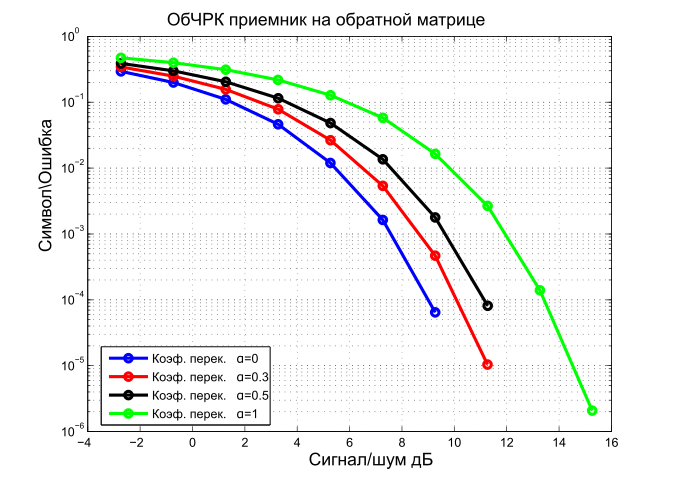
\includegraphics[width=0.9\columnwidth]{ZF_SER.png}
\caption{\textit{Зависимость производительности приемника от коэф. перекрытия $\alpha$ для приемника на псевдообратной матрице}}
\label{fs_1}
\end{figure}

\begin{figure}[H]
\centering
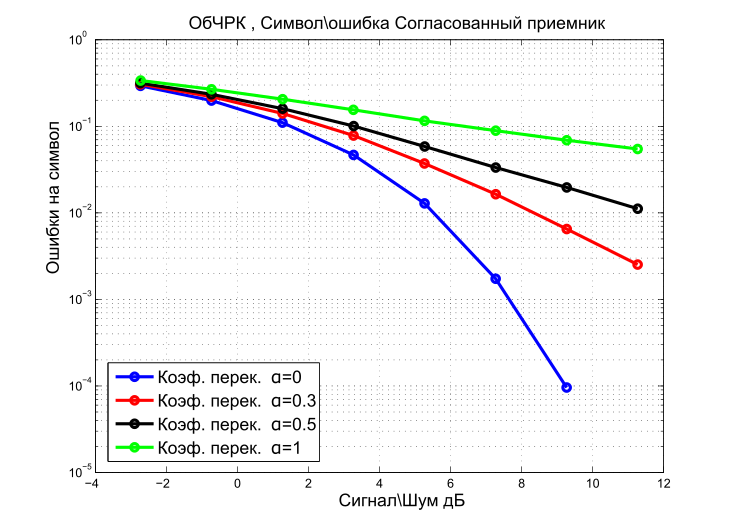
\includegraphics[width=0.9\columnwidth]{MF_SER.png}
\caption{\textit{Зависимость производительности приемника от коэф. перекрытия $\alpha$ для согласованного приемника}}
\label{fs_2}
\end{figure}
Производительность системы ОбЧРК для работы полу-слепого приемника получены при помощи моделирования. В системе был положен аддитивный белый Гауссов шум без какого либо кодирования. В системе была использована квадратурная фазовая манипуляция. Количество поднесущих равно $F=32$. Количество временных отсчетов на каждый временной символ равно $T/T_s=F$. Количество временных символов равно $T_s=15$. В качестве фильтра был использован фильтр с характеристикой "Корень из приподнятого косинуса" с коэффициентом перекрытия $\alpha=0.5$. Коэффициенты передачи для различных поднесущих были выбраны как случайные целочисленные величины в диапазоне от $0$ до $1$. На приемнике величины оцениваются как пороговые устройства и приравниваются разрешенным величинам. Результаты производительности системы ОбЧРК  показаны на двух рисунках, на первом рисунке показано соотношение символов к ошибкам в случае если приемник знает истинную величину вектора $\mathbf{a}$, при помощи приемника на псевдообратной матрице, если приемник если не знает истинную величину вектора $\mathbf{a}$.Кроме того показаны результаты работы двух версий полу-слепых приемников. На втором рисунке представлена нормализованная ошибку между истинным значением вектора истинную величину вектора $\mathbf{a}$ и найденным приемником.
\begin{table}[H]
\caption{\label{tab:sim_alpha}ОбЧРК эксперимент 1.2}
\begin{center}
\begin{tabular}{|c|c|c|}
\hline
Параметр & Обозначение & Значение \\
\hline
\hline
Вид модуляции & $\mu$ & КФМ-2 \\
\hline
Отсчетов на символ & $T/T_s$ & 32 \\
\hline
Поднесущие&$F$&32 \\
\hline
Разме блока передачи& $T_s$  &15 \\
\hline
Вид фильтра&  &КиПК \\
\hline
Коэффициент перекрытия&$\alpha$  &0.5 \\
\hline
Коэффициенты поднесущих& $\mathbf{a}_i$ & $randi([0 1])$ \\
\hline
Канал& $h$ &АБГШ \\
\hline
Префикс&  & Нет \\
\hline
Передача&  & Некодированно\\
\hline
\end{tabular}
\end{center}
\end{table}
\begin{figure}[H]
\centering
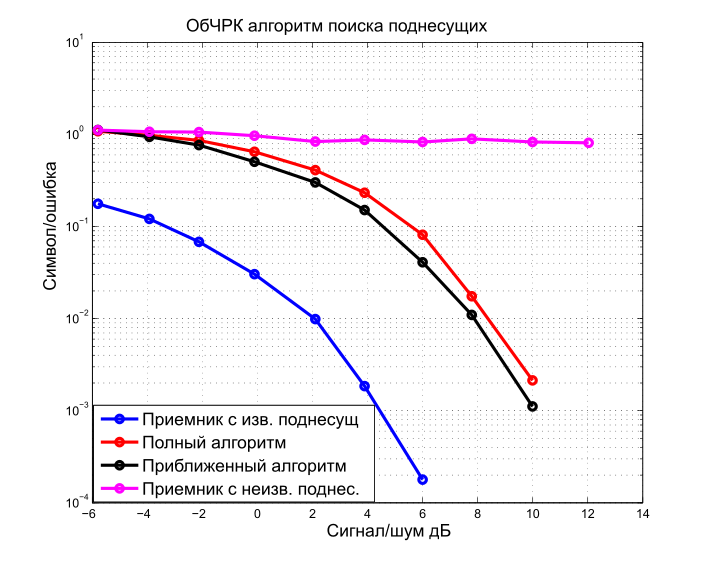
\includegraphics[width=0.9\columnwidth]{SM_SER.png}
\caption{\textit{Сравнение производительности для алгоритма поиска поднесущих}}
\label{fs_3}
\end{figure}
\begin{figure}[H]
\centering
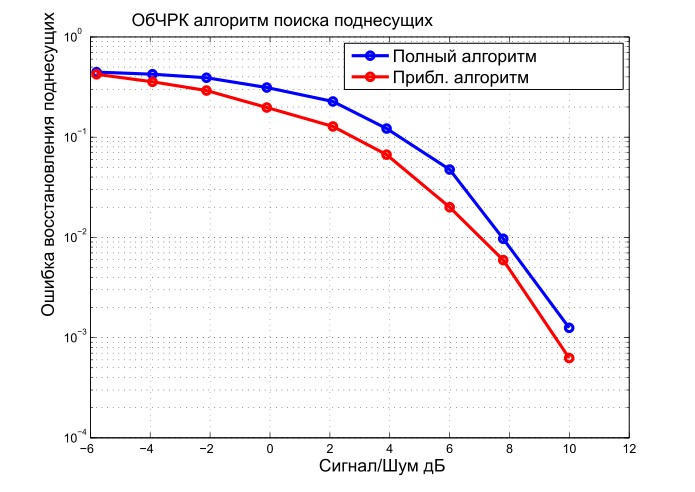
\includegraphics[width=0.9\columnwidth]{SM_RE.png}
\caption{\textit{Ошибка восстановления поднесущих}}
\label{fs_4}
\end{figure}
Кроме того мы добавили дополнительные графики для сравнения совместного и раздельного решения работы алгоритмов. Результаты сравнения так же получены при помощи моделирования.
\begin{table}[H]
\caption{\label{tab:sim_alpha}ОбЧРК эксперимент 1.3}
\begin{center}
\begin{tabular}{|c|c|c|}
\hline
Параметр & Обозначение & Значение \\
\hline
\hline
Сигнал/Шум & $log(P_s/P_n)$ & 10 \\
\hline
Отсчетов на символ & $T/T_s$ & 32 \\
\hline
Поднесущих&$F$&32 \\
\hline
Размер блока& $T_s$  &15 \\
\hline
Вид фильтра&  &КиПК \\
\hline
Коэффициент перекрытия&$\alpha$  &0.5 \\
\hline
Коэффициенты поднесущих& $randi([0 1])$ \\
\hline
\end{tabular}
\end{center}
\end{table}
\begin{figure}[H]
\centering
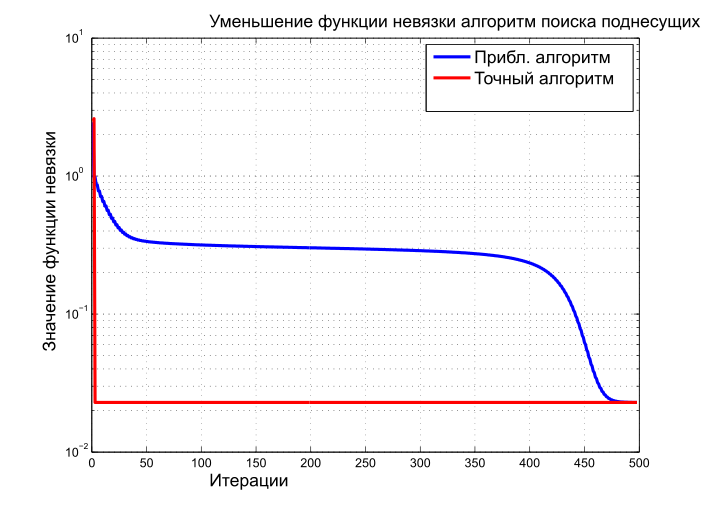
\includegraphics[width=0.9\columnwidth]{SM_conv.png}
\caption{\textit{Сходимость алгоритма по функции невязки}}
\label{fs_5}
\end{figure}
\begin{figure}[H]
\centering
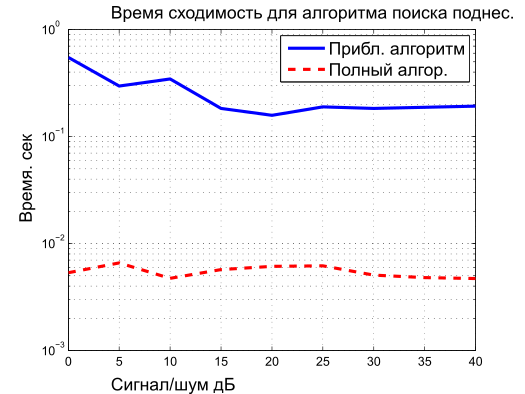
\includegraphics[width=0.9\columnwidth]{SM_TIME.png}
\caption{\textit{Время сходимости алгоритма в зависимости от соотношения сигнал/шум}}
\label{fs_6}
\end{figure}
\begin{figure}[H]
\centering
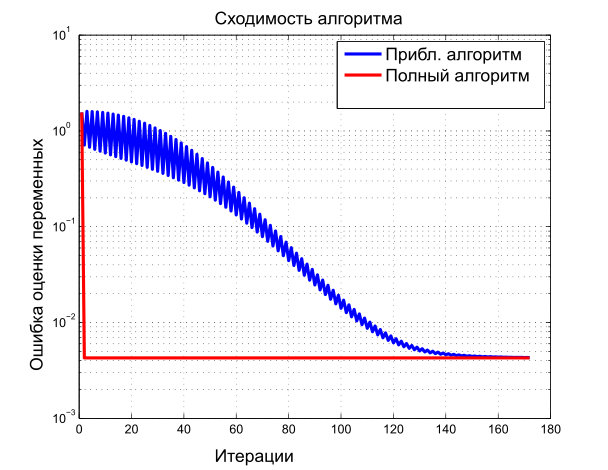
\includegraphics[width=0.9\columnwidth]{SM_RES.png}
\caption{\textit{Сходимость алгоритма по переменным}}
\label{fs_7}
\end{figure}
Производительность системы ОбЧРК для работы полу-слепого приемника получены при помощи моделирования. В системе был положен канал с памятью с дополнительным аддитивным белым Гауссовым шумом на входе приемника без какого либо кодирования. В системе была использована квадратурная фазовая манипуляция. Количество поднесущих равно $F=32$. Количество временных отсчетов на каждый временной символ равно $T/T_s=F$. Количество временных символов равно $T_s=32$. В качестве фильтра был использован фильтр с характеристикой "Корень из приподнятого косинуса" с коэффициентом перекрытия $\alpha=1$.  Результаты производительности системы ОбЧРК  показаны на двух рисунках, на первом рисунке показано соотношение символов к ошибкам для различного количества тренировочных символов и сравнение с приемником на обратной фильтрации. На втором рисунке представлена ошибка восстановления канала для различного количества тренировочных символов.

\begin{table}[H]
\caption{\label{tab:sim_alpha}ОбЧРК эксперимент 1.4}
\begin{center}
\begin{tabular}{|c|c|c|}
\hline
Параметр & Обозначение & Значение \\
\hline
\hline
Отсчетов на символ & $T/T_s$ & 32 \\
\hline
Поднесущих&$F$&32 \\
\hline
Размер блока& $T_s$  &15 \\
\hline
Вид фильтра&  &КиПК \\
\hline
Коэффициент перекрытия&$\alpha$  &1 \\
\hline
Тип канала& $Ped-A$ \\
\hline
\end{tabular}
\end{center}
\end{table}
\begin{figure}[H]
\centering
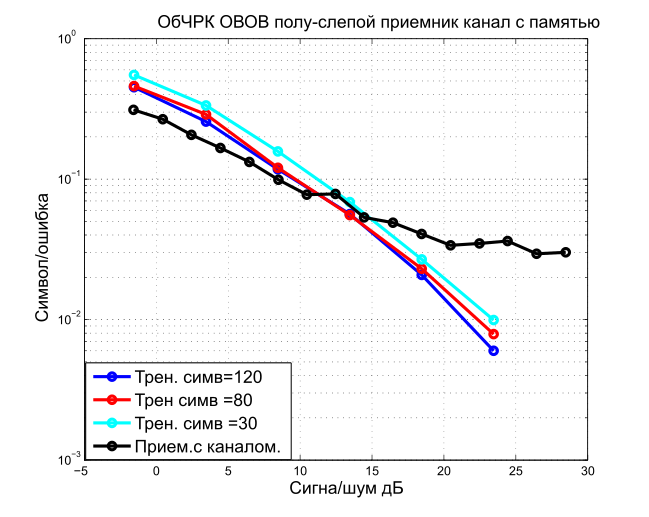
\includegraphics[width=0.9\columnwidth]{SM_SISO_FS_SER.png}
\caption{\textit{Производительность работы полу-слепого приемника от сигнал/шум и количества тренировочных символов}}
\label{fs_8}
\end{figure}
\begin{figure}[H]
\centering
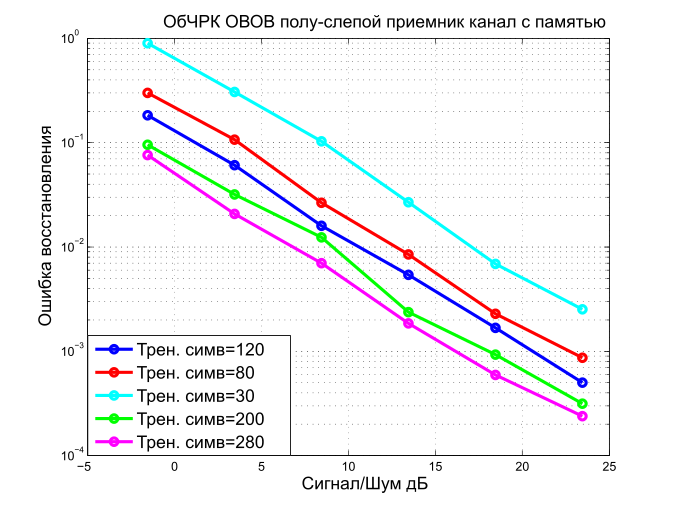
\includegraphics[width=0.9\columnwidth]{SM_SISO_FS_RE.png}
\caption{\textit{Ошибка восстановления канала полу-слепого приемника от сигнал/шум и количества тренировочных символов}}
\label{fs_9}
\end{figure}
\section{Заключение}
В качестве заключение по первому эксперименту мы можем сказать, что приемник на основе псевдообратной матрицы показывает значительно лучшие результаты в детектировании символов по сравнению с согласованными приемником. Разница между приемниками незначительная в случае если коэффициент перекрытия имеет малое значение. Однако увеличение коэффициента перекрытия значительно уменьшает производительность системы на основе согласованного фильтра. Это связано с тем, что увеличивается перекрытие по частоте $\alpha$ между поднесущими. Таким образом из рис.\ref{fs_1} видно что увеличение коэффициента перекрытия до максимума уменьшает производительность системы на 5 дБ. При этом производительность системы на основе согласованного фильтра значительно ухудшается, что видно на рис.\ref{fs_2} и делает применение согласованного фильтра бесполезным. Таким образом результаты показывают, что предпочтительнее использовать приемник на основе псевдо-обратной матрицы. Таким образом можно обеспечить лучшие результаты по вне-полосным излучениям системы при этом устранять влияние взаимной интерференции в системе. Более того можно использовать дополнительные алгоритмы для устранения взаимной интерференции в системе позволяющие получить дополнительное увеличение производительности.
В качестве заключения для эксперимента с анализом алгоритма оценки работающих подчастот можно сделать следующие выводы :
\begin{itemize}
\item Алгоритм позволяет определить была ли включена поднесущая и передавались ли по ней данные.
\item Использование алгоритма приводит к ухудшению производительности системы на 5-6дБ.
\item Алгоритм может быть доработан использованием дополнительных техник по принятию решения о том, была ли включена поднесущая.
\end{itemize}
Как сказано в п.1 алгоритм работает и позволяет автоматически, без вероятностных моделей определить были ли переданы данные по поднесущей, при условии что для приемника известен хотя бы один символ на каждой из поднесущих. Однако применение системы при сравнении со случаем, когда приемник идеально знает используемые поднесущие приводит к ухудшению производительности на 5 дБ что показано на рис.\ref{fs_3}. Данное снижение в производительности связано с тем, что увеличивается количество источников ошибок, и в случае если приемник ошибочно определил поднесущую как включенную, это приводит к большому количеству ошибок. При этом цена ошибки принятия решения оказывается высокой, в то время как в функцию невязки оба выражения входят с одинаковым коэффициентом. В качестве решающего устройства было использовано пороговое устройство оценивавшее абсолютную величину коэффициента поднесущей, в случае если величина была больше 0.5 поднесущая считалась включенной. Поскольку данное решение не является оптимальным, возможно применение иных техник для увеличения эффективности алгоритма. Кроме того как показывают результаты на рис.\ref{fs_3}и рис.\ref{fs_4} , приближенный алгоритм имеет производительность лучше, чем у алгоритма с полной точностью. Это может быть связано с тем, что приближенное решение  имеет тенденцию к ошибкам типа "пропуск сигнала", и поскольку было оценено меньшее количество поднесущих чем на самом деле было использовано, то и количество соответствующих ошибок окажется меньше. Таким образом с точки зрения данной метрики производительность является большей, однако она является несущественной. Так же дополнительные рисунки показывают преимущества алгоритма с полной точностью. Как видно из рис.\ref{fs_5}. Скорость сходимости алгоритмов отличается значительно. Алгоритм полной точности сходится всего за две итерации, что позволяет уменьшить количество вычислений во много раз, в то время как алгоритм  приближенной точности требует в среднем 100-200 итераций для сходимости. Таким образом последующая зависимость времени сходимости алгоритма на рис. \ref{fs_6} оказывается значительно лучше у алгоритма полной точности из-за количества итераций приближенного алгоритма. При этом даже, тот факт, что каждая итерация алгоритма приближенной точности требует меньше вычислительных ресурсов, в итоге алгоритм затрачивает значительно больше  ресурсов. Как можно видеть из рис. \ref{fs_7} сходимость алгоритма приближенной точности происходит нелинейно и достаточно нестабильно, вызывая колебания ошибки восстановления на каждой итерации. Это вызывает долгий итерационный процесс, что и является следствием столь долгой сходимости алгоритма.

Эксперимент по проверке работы полу слепого приемника оценивающего состояние канала и принятые символы показывает следующие результаты:
\begin{itemize}
\item Правильным образом выбирая известные символы в блоке данных можно достичь даже лучшей производительности, чем если идеально знать канал и делать поиск по всем возможным символам.
\item Алгоритм показывает хорошую производительность по каналу пешеходного типа А. 
\item Производительность алгоритма зависит от количества неизвестных символов.
\end{itemize}
Как видно из рис. производительность системы  полу-слепым приемником на основе оптимизации показывает результат лучше, чем даже если был бы использован приемник на основе обратной фильтрации с идеально известным каналом, что говорит о больше стабильности алгоритма. Однако подобное поведение будет изменяться в случае если будут включены только некоторые поднесущие. Производительность системы меняется в зависимости от того сколько символов в блоке данных известно для приемника. После некоторой величины производительность системы падает ниже уровня приемника с идеально известным каналом. Таким образом можно адаптивно регулировать производительность системы. Как видно из рис. кривые ошибки восстановления канала лежат параллельно друг другу позволяя так же адаптивно выбирать точность определения канала гибко, таким образом обновляя состояние канала если он не меняется и уменьшать количество символов на первой итерации для более точного определения канала. Кроме того благодаря использованному подходу с вычитанием известных символов из функции невязки взаимная интерференция между разными каналами так же уменьшается и дополнительно увеличивает производительность системы. Кроме того в случае постановки задачи оптимизации количества излучаемой энергии к количеству полученной информации будет получена вогнутая кривая производительности по качеству работы системы в зависимости от количества известным системе символов.
Основным выводом можно считать что данный подход является чрезвычайно эффективным с точки зрения качества работы системы, однако не является реализуемым на практике с точки зрения оборудования, так как потребует значительных вычислительных ресурсов, однако возможна параллельная обработка принятых данных, что вероятно может ускорить работу системы. Более того для простых задач с небольшими объемами данных современные встроенные системы могут реализовать данные операции.
\clearpage

\cleardoublepage
%\addcontentsline{toc}{chapter}{Список литературы}
\bibliographystyle{utf8gost705u}  
\bibliography{art1} 
\cleardoublepage
\end{document}

%\selectlanguage{russian}